%--------------------------------------------------------------
%Preamble
%\documentclass[a4paper, twoside, 11pt]{book}
\documentclass[twoside,openany,11pt]{book}
\usepackage[%
  papersize={210mm,297mm},%
  layoutsize={200mm,294mm},%
  layoutoffset=5mm,%
  twoside,%
  nomarginpar,%
  inner=20mm,%
  outer=20mm,%
  vmargin=25mm,%
  voffset=0mm,
  head=20mm,%
  headsep=10mm,%
  includefoot,
  foot=0mm,%
  %includefoot,
  %showcrop,%
  %showframe,%
]{geometry}
\setlength{\parindent}{0mm}
\setlength{\parskip}{1mm plus 0.5mm minus 0.5mm}
\setlength{\topskip}{5mm}
\setlength{\textfloatsep}{4mm}

\usepackage[pdftex, final]{graphicx}
\graphicspath{{./pics/}}
\usepackage[parfill]{parskip}
\usepackage{microtype}
\usepackage{amssymb}
\usepackage{amsmath}
\usepackage{mathtools}
\usepackage{bm}
\usepackage{tensor}
\usepackage{titlesec}
\newcommand{\sectionbreak}{\clearpage}
\usepackage[linesnumbered,lined,boxed,commentsnumbered,ruled]{algorithm2e}
\setcounter{tocdepth}{6}
\setcounter{secnumdepth}{6}
%\setcounter{chapter}{1}
%\usepackage{enumitem}
%\setlist{nosep} % or \setlist{noitemsep} to leave space around whole list

\usepackage{subfigure}
%filepath for figures
\graphicspath{{./figures/}}

%tikz
\usepackage{tikz,tikz-3dplot} 
%\usetikzlibrary{calc}
\tdplotsetmaincoords{60}{-25}
\usepackage{verbatim}
\usepackage{amsmath}
\DeclareMathOperator*{\argmin}{arg\,min}
\usetikzlibrary{arrows,positioning} 
\tikzset{
    %Define standard arrow tip
    >=stealth',
    %Define style for boxes
    punkt/.style={
           rectangle,
           rounded corners,
           draw=black, very thick,
           text width=6.5em,
           minimum height=2em,
           text centered},
    % Define arrow style
    pil/.style={
           ->,
           thick,
           shorten <=2pt,
           shorten >=2pt,}
}

%--------------------------------------------------------------
\begin{document}

\title{Title}
\author{Montiel Abello}
%\date{\vspace{-5ex}}
\date{}  % Toggle commenting to test
\maketitle

\chapter*{Acknowledgements}
\addcontentsline{toc}{chapter}{Acknowledgments}

I would like to thank my supervisors Dr Jochen Trumpf and Dr Viorela for all the guidance they gave. Thank you for being so generous with your time and providing so much encouragement and support.


\chapter*{Abstract}
\addcontentsline{toc}{chapter}{Abstract}

The aim of this research was to design and implement an observer to estimate the state of a rigid cube from sparse range measurements. This was motivated by active research in the development of a design methodology for symmetry-preserving, infinite dimensional observers. The simplified cube estimation problem serves as a first step in this research direction, investigating the use of a sparse sensor in dense estimation and identifying effective innovation functions for rigid body state estimation. 

A Matlab toolbox was developed to simulate measurements of rigid bodies by a Hokuyo UBG-04LX-F01 scanning laser range-finder. This simulation was used to assess the performance of the observer. Experimental data was collected to more realistically simulate the error distribution of the sensor and for future testing of observers under real-world conditions. 

The simulation results show that the observer is globally convergent when correcting orientation and size error. An $\mathbf{SE}(3)$ invariant innovation function would be required to concurrently correct position and orientation, showing the importance of symmetry considerations in nonlinear observer design. This research also demonstrates that dense estimation can performed using sparse range measurements, given a suitable sensor trajectory. 



\markboth{Contents}{Contents}
\tableofcontents
\listoffigures

\chapter{Introduction}

Advances in manufacturing and hardware design have made mobile robots more accessible for not only research and industrial purposes, but to the general public. However, autonomous robots have largely been limited to indoor, carefully controlled environments. Before autonomous robots can be more widely deployed, they must be able to accurately observe and represent unstructured, dynamic environments. Dense sensors such as light field cameras are becoming cheaper and lighter, promising to allow autonomous robots to acquire detailed measurements of complex environments. To fully utilise the potential of these advancing technologies, improvements in observer design are required to generate more accurate and detailed descriptions of these environments from dense measurements.

One method of estimating the state of a complex environment is with an \textit{infinite-dimensional observer}. Typically, observers for infinite-dimensional systems are extensions of finite-dimensional Luenberger observers. Unfortunately, this design approach is only able to guarantee convergence for linear systems. Developing a theory of symmetry-preserving, infinite-dimensional observers would simplify the design process for nonlinear systems and result in observers with improved convergence properties.

This research project serves as an initial exploration into the design of symmetry-preserving, infinite-dimensional observers. An observer for a simplified system will be designed and implemented. The potential for a symmetry-preserving, infinite-dimensional observer to improve performance will be explored. 

This report presents the novel implementation of an observer to estimate the state of a rigid cube from range measurements. Section \ref{sec:literature} reviews the current state of observer design methods for infinite-dimensional systems. Recent work in the development of design methodologies for symmetry preserving observers is described. Particular attention is paid to a dense optical flow estimator that will be particularly relevant to this research.
 
Chapter \ref{chap:background} provides theory on Lie groups, rigid body state representation and state observer concepts that will be relevant in the observer design.

The cube state estimation problem that is the focus of this research is described in detail in Chapter \ref{chap:problem}. The place of this problem within the larger area of symmetry-preserving, infinite-dimensional observer research is defined.  

Chapter \ref{chap:simulation} provides a detailed description of the simulation implementation, including the observer update function design. The performance of the observer in estimating the state of stationary and moving cubes is assessed. It is shown that almost global convergence is achieved for orientation and size correction for stationary cubes, though the position update only converges in special cases.

Chapter \ref{chap:experiment} details steps taken to experimentally validate the results of the simulation. Range measurement data is collected and used to develop an error distribution model for the Hokuyo UBG-04LX-F01 sensor. Range measurements of a cube of known trajectory are taken for future performance testing.

\section{Literature review} \label{sec:literature}
The use of dense sensors allows for a more accurate estimation of the state of an infinite-dimensional system such as a complex, real-world environment. The theory of infinite-dimensional observers is required to fully utilise this information. This section will review the current state of design methodologies and implementations for infinite-dimensional observers. Particular focus will be paid to an emerging avenue of research; symmetry-preserving observer design. Recent theory developments in this area have allowed limitations in the global convergence properties of nonlinear observers to be overcome.

\subsection{Infinite-dimensional observers}
In many real world systems the dependent variables are functions of one or more spatial variables. An example would be the dynamics of waves in a body of water. The height of the surface varies continuously along the $x$ and $y$ directions. These spatial variables vary continuously, meaning an infinite number of parameters is required to describe the state of the system. Such systems are termed \textit{infinite-dimensional systems}, or \textit{distributed parameter systems}. Their dynamics are modelled by a partial differential equation (PDE). 

When a state estimate is required but direct measurement of the state with sensors is difficult or impossible, a \textit{state observer} is employed. A state observer is a filter that provides an estimate of the state of a system using the difference between its measured and predicted outputs. A more detailed description of the concept of a state observer is provided in Section \ref{sec:observerequations}. An observer for an infinite-dimensional system is called an \textit{infinite-dimensional observer}.

\subsubsection{Linear systems}
Observer theory for \textit{linear} infinite-dimensional systems has been widely studied. The techniques used are typically extensions of Luenberger observers and Kalman filter methods used to observe finite dimensional system.

A simplified approach is to use a spatial discretisation method such as finite difference or finite element to reduce the infinite-dimensional system to a finite-dimensional one. From here, finite-dimensional observer design techniques can be used. This is known as the \textit{early lumping} method, and was employed by Stavroulakis \cite{stavroulakis1973design} who implemented a finite-dimensional observer as part of a control system for an infinite dimensional systems.

The early lumping approach suffers from \textit{spillover}, a phenomenon where performance is affected by the neglected dynamics of the system\cite{meirovitch1983problem}. Harkort \cite{harkort2011finite} recently developed an observer based control scheme that reduced this effect by using modelled outputs rather than true measurements to reduce the effect of the neglected dynamics.

More accurate observers can be designed with the \textit{late lumping} approach which uses the infinite-dimensional model of the system in the observer design. The result is an infinite-dimensional observer that is discretised later for practical implementation. These methods are typically extensions of Kalman or Luenberger methods to infinite dimensions. 

Early work by Gressang \cite{gressang1975observers} extended the Luenberger observer to infinite-dimensional systems whose state space was an abstract Banach space with dynamics defined by an infinitesimal generator of a semigroup. More recently, Smyshlyaev \cite{smyshlyaev2005backstepping} developed an exponentially converging backstepping observer for systems governed by parabolic PDEs. Ramdani introduced forward and backward observers \cite{ramdani2010recovering} whose convergence properties were investigated by Haine \cite{haine2014recovering}.

\subsubsection{Nonlinear systems}
There is currently no universal approach for observer design for nonlinear infinite-dimensional systems.
The most common approach has been to linearise the system, then apply a linear infinite-dimensional observer design. Common linearisation methods include Lyapunov methods, extended linearisation and the Lie-algebraic approach \cite{primbs1996survey}.

There has been some progress in infinite-dimensional observer design for special cases of nonlinear systems. For bilinear systems, Xu \cite{xu1995observer} designed an infinite-dimensional observer that converged for certain inputs. Bounit \cite{bounit1997observers} designed Kalman and Luenberger type observers for infinite-dimensional bilinear systems. 

Despite these small advances in special cases of nonlinear design, the most common design methods for nonlinear infinite-dimensional systems are based on linearisation techniques. These techniques rely on the fact that differentiable functions can be approximated by a first-order Taylor expansion around a point. Luenberger and Kalman methods can be applied to linear approximations of infinite-dimensional systems around an equilibrium point. This simplification relies on the dynamics of system at the point of linearisation being representative of the entire space. In general, this is not necessarily true, and is the biggest limitation in this design technique. The result is that these linearised observers only converge if the initial state estimate is within a local neighbourhood of the true state. Global converge is not guaranteed which severely limits robustness.

Global convergence can be achieved by taking account the symmetries inherent to the system during observer design. A powerful tool for dealing with symmetries is the theory of \textit{Lie groups}. Investigation into \textit{symmetry-preserving} observer design for systems on Lie groups is an active area of research. It promises to produce theoretically validated design principles for nonlinear infinite-dimensional observers, though the majority of research so far has been limited to finite-dimensional observers.

\subsection{Symmetry-preserving observers}
The motivation behind symmetry-preserving observers is to take advantage of invariances in the dynamics of the system. The goal is to design an observer around an equilibrium point in such a way that it can be extended to converge around a wider set of points.

\subsubsection{Early work}
Geometry conscious observer design is not a new idea. Early investigation by Marcus \cite{marcus1984algebraic} into algebraic and geometric methods for nonlinear filter design showed promise.
A seminal work by Salcudean \cite{salcudean1991globally} was the design of an eventually-exponential, globally converging observer for the attitude of rigid bodies from orientation and torque measurements. This observer design took advantage of the simplicity of the quaternion rotation representation and dynamics of rigid body motion.

Another important result that is a precursor to the active research of today is a design method developed by Aghannon \& Rouchon \cite{aghannan2002invariant}. Their invariant observer construction was based on Cartan's moving frame method. Though convergence was proven for a specific problem, the observer convergence for a general case was left an open problem. Maithripala \cite{maithripala2005intrinsic} demonstrated the effectiveness of Aghannon \& Rouchons' method by incorporating it into the design of an intrinsic observer based controller. Performance was shown to be independent of the coordinate system used to represent the configuration space.

\subsubsection{Active research}
There are currently two groups actively researching symmetry-preserving observer design.  Both have begun to apply symmetry-preserving methods to infinite-dimensional observers.

The work of Bonnabel, Auroux, Rouchon, Martin et al. is a progression of the early results from Aghannon \& Rouchon. Their general approach is to first design a Luenberger type observer around an equilibrium point. An invariant frame is used to construct an invariant output error. The observer innovation term respects the symmetries of the system and thus the nonlinear observer is well behaved around a continuum of equilibrium points. 

In \cite{bonnabel2005invariant}, Bonnabel et a. developed an observer design procedure based on Aghannon \& Rouchons' work. Asymptotic stability was achieved, though this required a design procedure tailored to specific nonlinearities of the system and did not apply in a general case.
It was shown in \cite{bonnabel2008symmetry} that an invariant error equation simplified convergence analysis. The observer's global behaviour improved, having a larger region of attraction in comparison to naively linearised observers.
Developments were made to the theory and presented in \cite{bonnabel2009non}. For a particular class of invariant system it was shown that the observer converged locally around any trajectory, and global convergence behaviour was independent of trajectory.

Most recently, these invariant design methods were applied to an infinite dimensional system \cite{auroux2011symmetry}. An observer estimating the state of fluid in a water tank where height varied with the continuous dependent variables position and time was developed. It was shown to converge more quickly and robustly than previous attempts to design infinite dimensional observers with Extended Kalman Filter (EKF) methods.

The work of Trumpf, Mahony, Hamel, Lageman et al. differs in scope. The methods of Bonnabel et al. are generalised and can be applied to a wide range of systems. In contrast, the work of Trumpf et al. is limited to two specific classes of systems but achieves stronger convergence properties.
In \cite{mahony2009nonlinear} nonlinear filters on the Special Orthogonal Group $\mathbf{SO}(3)$ are used in attitude estimation and the resulting nonlinear observers achieved almost globally stable observer error.
Another attitude observer \cite{trumpf2012analysis} achieved almost globally asymptotic and locally exponential convergence.
In \cite{mahony2013observers}, the design methodology for 2 classes of systems is presented. The approach taken is to lift the kinematic system onto its symmetry group and design an observer for the lifted system. The Lyapunov method is used to design the observer innovation term. This methodology simplifies nonlinear observer design and produces observers with strong convergence properties. This group has also begun research  on symmetry-preserving infinite-dimensional observers.

The motivation behind the development of infinite-dimensional observers is to allow dense sensors to be fully utilised. In this vein, research presented in a PhD thesis by Zarrouati \cite{zarrouati2013augmented} utilised dense measurements from a camera and depth sensor. An observer was developed from rotation invariant equations for light and depth. Though the sensors took measurements of an infinite dimensional state, a finite dimensional approximation of this state is what was estimated by the observer.

Another recent work by Adarve et al.\cite{adarvefiltering} also uses dense sensing in the estimation of an infinite dimensional state. This result will be examined closely as it is similar in direction to this research.

Adarve et al. design an update-propagation filter to iteratively compute dense optical flow $\Phi$ from CCD camera measurements $Y$. In reality, this optical flow is an infinite dimensional state. Rather than computing the optical flow independently at each frame, a two-stage process is used to build it incrementally. The propagation stage uses a non-linear PDE to model the transport of the optical flow in the next time step. The update stage corrects this prediction using the current image.

The iterative filter used in this approach is an observer that estimates the state of the continuous spatio-temporal flow field. By using a dense sensor, the measured image stream can be treated as a continuous, infinite-dimensional state. This is in contrast to sparse optical flow computation where the image is modelled as a set of discrete pixel values. However, the flow field $\Phi$ is discretised and computed in $r$ independent regions $\Omega$ around a discrete set of control points $\xi$ as shown in Figure \ref{fig:flow}. Here, this approach differs from that of general infinite-dimensional invariant observer. The state is treated as a discrete set of locally continuous states which does not allow for symmetry considerations. This is because the PDE relations in the local regions are invariant to 2D rotation and translation, but the interactions between regions themselves are not. 

\begin{figure}
\centering
  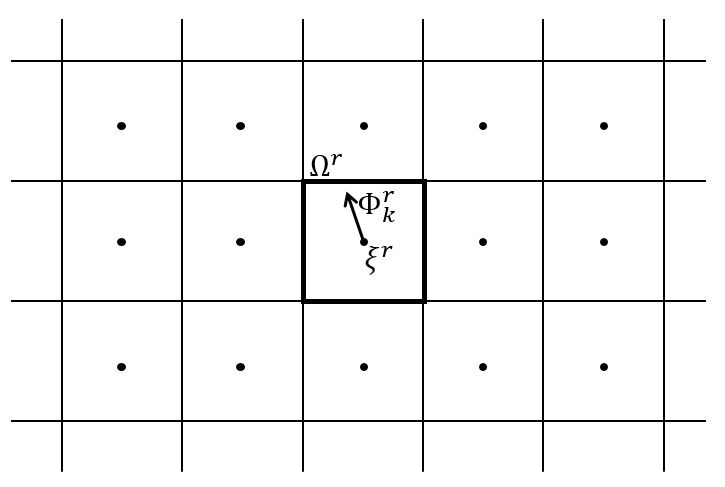
\includegraphics[width=0.8\textwidth,trim = 0mm 0mm 0mm 0mm,clip]{./Figures/flow_regions.jpg}
  \caption{Infinite dimensional optical flow discretised and computed in separate, independent regions} \label{fig:flow_regions}
\end{figure} \label{fig:flow}

Discretising $\Phi$ and $Y$ at the beginning of the algorithm design makes this is an example of the early lumping design approach. Employing a late lumping approach by discretising an infinite dimensional observer would allow for the rotation and translation invariance of the flow field to be taken advantage of to improve convergence properties. 

The lesson to take from this analysis is that discretisation methods must be carefully chosen in order to preserve the invariance of the observer.

Another reason to pay attention to geometric symmetries in observer design is due to limitations placed on convergence by the topology of the system. Bhat \& Bernstein \cite{bhat2000topological} show that global convergence cannot be achieved with a continuous observer on a state space that includes a vector bundle such as $\mathbf{SE}(3)$. Some advancements have been made with extended state-space observers \cite{huang2000analysis,talole2010extended}, that extend the state space. However, this scheme can produce state estimates that are incompatible with the physics of the system prior to convergence. A theory of symmetry-preserving observer design for infinite dimensional systems could simplify observer design and convergence analysis for such systems.



\section{Literature review} \label{sec:literature}
The use of dense sensors allows for a more accurate estimation of the state of an infinite-dimensional system such as a complex, real-world environment. The theory of infinite-dimensional observers is required to fully utilise this information. This section will review the current state of design methodologies and implementations for infinite-dimensional observers. Particular focus will be paid to an emerging avenue of research; symmetry-preserving observer design. Recent theory developments in this area have allowed limitations in the global convergence properties of nonlinear observers to be overcome.

\subsection{Infinite-dimensional observers}
In many real world systems the dependent variables are functions of one or more spatial variables. An example would be the dynamics of waves in a body of water. The height of the surface varies continuously along the $x$ and $y$ directions. These spatial variables vary continuously, meaning an infinite number of parameters is required to describe the state of the system. Such systems are termed \textit{infinite-dimensional systems}, or \textit{distributed parameter systems}. Their dynamics are modelled by a partial differential equation (PDE). 

When a state estimate is required but direct measurement of the state with sensors is difficult or impossible, a \textit{state observer} is employed. A state observer is a filter that provides an estimate of the state of a system using the difference between its measured and predicted outputs. A more detailed description of the concept of a state observer is provided in Section \ref{sec:observerequations}. An observer for an infinite-dimensional system is called an \textit{infinite-dimensional observer}.

\subsubsection{Linear systems}
Observer theory for \textit{linear} infinite-dimensional systems has been widely studied. The techniques used are typically extensions of Luenberger observers and Kalman filter methods used to observe finite dimensional system.

A simplified approach is to use a spatial discretisation method such as finite difference or finite element to reduce the infinite-dimensional system to a finite-dimensional one. From here, finite-dimensional observer design techniques can be used. This is known as the \textit{early lumping} method, and was employed by Stavroulakis \cite{stavroulakis1973design} who implemented a finite-dimensional observer as part of a control system for an infinite dimensional systems.

The early lumping approach suffers from \textit{spillover}, a phenomenon where performance is affected by the neglected dynamics of the system\cite{meirovitch1983problem}. Harkort \cite{harkort2011finite} recently developed an observer based control scheme that reduced this effect by using modelled outputs rather than true measurements to reduce the effect of the neglected dynamics.

More accurate observers can be designed with the \textit{late lumping} approach which uses the infinite-dimensional model of the system in the observer design. The result is an infinite-dimensional observer that is discretised later for practical implementation. These methods are typically extensions of Kalman or Luenberger methods to infinite dimensions. 

Early work by Gressang \cite{gressang1975observers} extended the Luenberger observer to infinite-dimensional systems whose state space was an abstract Banach space with dynamics defined by an infinitesimal generator of a semigroup. More recently, Smyshlyaev \cite{smyshlyaev2005backstepping} developed an exponentially converging backstepping observer for systems governed by parabolic PDEs. Ramdani introduced forward and backward observers \cite{ramdani2010recovering} whose convergence properties were investigated by Haine \cite{haine2014recovering}.

\subsubsection{Nonlinear systems}
There is currently no universal approach for observer design for nonlinear infinite-dimensional systems.
The most common approach has been to linearise the system, then apply a linear infinite-dimensional observer design. Common linearisation methods include Lyapunov methods, extended linearisation and the Lie-algebraic approach \cite{primbs1996survey}.

There has been some progress in infinite-dimensional observer design for special cases of nonlinear systems. For bilinear systems, Xu \cite{xu1995observer} designed an infinite-dimensional observer that converged for certain inputs. Bounit \cite{bounit1997observers} designed Kalman and Luenberger type observers for infinite-dimensional bilinear systems. 

Despite these small advances in special cases of nonlinear design, the most common design methods for nonlinear infinite-dimensional systems are based on linearisation techniques. These techniques rely on the fact that differentiable functions can be approximated by a first-order Taylor expansion around a point. Luenberger and Kalman methods can be applied to linear approximations of infinite-dimensional systems around an equilibrium point. This simplification relies on the dynamics of system at the point of linearisation being representative of the entire space. In general, this is not necessarily true, and is the biggest limitation in this design technique. The result is that these linearised observers only converge if the initial state estimate is within a local neighbourhood of the true state. Global converge is not guaranteed which severely limits robustness.

Global convergence can be achieved by taking account the symmetries inherent to the system during observer design. A powerful tool for dealing with symmetries is the theory of \textit{Lie groups}. Investigation into \textit{symmetry-preserving} observer design for systems on Lie groups is an active area of research. It promises to produce theoretically validated design principles for nonlinear infinite-dimensional observers, though the majority of research so far has been limited to finite-dimensional observers.

\subsection{Symmetry-preserving observers}
The motivation behind symmetry-preserving observers is to take advantage of invariances in the dynamics of the system. The goal is to design an observer around an equilibrium point in such a way that it can be extended to converge around a wider set of points.

\subsubsection{Early work}
Geometry conscious observer design is not a new idea. Early investigation by Marcus \cite{marcus1984algebraic} into algebraic and geometric methods for nonlinear filter design showed promise.
A seminal work by Salcudean \cite{salcudean1991globally} was the design of an eventually-exponential, globally converging observer for the attitude of rigid bodies from orientation and torque measurements. This observer design took advantage of the simplicity of the quaternion rotation representation and dynamics of rigid body motion.

Another important result that is a precursor to the active research of today is a design method developed by Aghannon \& Rouchon \cite{aghannan2002invariant}. Their invariant observer construction was based on Cartan's moving frame method. Though convergence was proven for a specific problem, the observer convergence for a general case was left an open problem. Maithripala \cite{maithripala2005intrinsic} demonstrated the effectiveness of Aghannon \& Rouchons' method by incorporating it into the design of an intrinsic observer based controller. Performance was shown to be independent of the coordinate system used to represent the configuration space.

\subsubsection{Active research}
There are currently two groups actively researching symmetry-preserving observer design.  Both have begun to apply symmetry-preserving methods to infinite-dimensional observers.

The work of Bonnabel, Auroux, Rouchon, Martin et al. is a progression of the early results from Aghannon \& Rouchon. Their general approach is to first design a Luenberger type observer around an equilibrium point. An invariant frame is used to construct an invariant output error. The observer innovation term respects the symmetries of the system and thus the nonlinear observer is well behaved around a continuum of equilibrium points. 

In \cite{bonnabel2005invariant}, Bonnabel et a. developed an observer design procedure based on Aghannon \& Rouchons' work. Asymptotic stability was achieved, though this required a design procedure tailored to specific nonlinearities of the system and did not apply in a general case.
It was shown in \cite{bonnabel2008symmetry} that an invariant error equation simplified convergence analysis. The observer's global behaviour improved, having a larger region of attraction in comparison to naively linearised observers.
Developments were made to the theory and presented in \cite{bonnabel2009non}. For a particular class of invariant system it was shown that the observer converged locally around any trajectory, and global convergence behaviour was independent of trajectory.

Most recently, these invariant design methods were applied to an infinite dimensional system \cite{auroux2011symmetry}. An observer estimating the state of fluid in a water tank where height varied with the continuous dependent variables position and time was developed. It was shown to converge more quickly and robustly than previous attempts to design infinite dimensional observers with Extended Kalman Filter (EKF) methods.

The work of Trumpf, Mahony, Hamel, Lageman et al. differs in scope. The methods of Bonnabel et al. are generalised and can be applied to a wide range of systems. In contrast, the work of Trumpf et al. is limited to two specific classes of systems but achieves stronger convergence properties.
In \cite{mahony2009nonlinear} nonlinear filters on the Special Orthogonal Group $\mathbf{SO}(3)$ are used in attitude estimation and the resulting nonlinear observers achieved almost globally stable observer error.
Another attitude observer \cite{trumpf2012analysis} achieved almost globally asymptotic and locally exponential convergence.
In \cite{mahony2013observers}, the design methodology for 2 classes of systems is presented. The approach taken is to lift the kinematic system onto its symmetry group and design an observer for the lifted system. The Lyapunov method is used to design the observer innovation term. This methodology simplifies nonlinear observer design and produces observers with strong convergence properties. This group has also begun research  on symmetry-preserving infinite-dimensional observers.

The motivation behind the development of infinite-dimensional observers is to allow dense sensors to be fully utilised. In this vein, research presented in a PhD thesis by Zarrouati \cite{zarrouati2013augmented} utilised dense measurements from a camera and depth sensor. An observer was developed from rotation invariant equations for light and depth. Though the sensors took measurements of an infinite dimensional state, a finite dimensional approximation of this state is what was estimated by the observer.

Another recent work by Adarve et al.\cite{adarvefiltering} also uses dense sensing in the estimation of an infinite dimensional state. This result will be examined closely as it is similar in direction to this research.

Adarve et al. design an update-propagation filter to iteratively compute dense optical flow $\Phi$ from CCD camera measurements $Y$. In reality, this optical flow is an infinite dimensional state. Rather than computing the optical flow independently at each frame, a two-stage process is used to build it incrementally. The propagation stage uses a non-linear PDE to model the transport of the optical flow in the next time step. The update stage corrects this prediction using the current image.

The iterative filter used in this approach is an observer that estimates the state of the continuous spatio-temporal flow field. By using a dense sensor, the measured image stream can be treated as a continuous, infinite-dimensional state. This is in contrast to sparse optical flow computation where the image is modelled as a set of discrete pixel values. However, the flow field $\Phi$ is discretised and computed in $r$ independent regions $\Omega$ around a discrete set of control points $\xi$ as shown in Figure \ref{fig:flow}. Here, this approach differs from that of general infinite-dimensional invariant observer. The state is treated as a discrete set of locally continuous states which does not allow for symmetry considerations. This is because the PDE relations in the local regions are invariant to 2D rotation and translation, but the interactions between regions themselves are not. 

\begin{figure}
\centering
  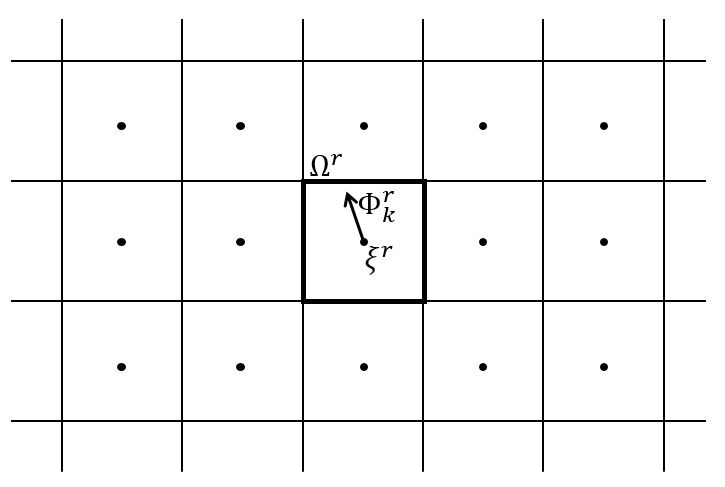
\includegraphics[width=0.8\textwidth,trim = 0mm 0mm 0mm 0mm,clip]{./Figures/flow_regions.jpg}
  \caption{Infinite dimensional optical flow discretised and computed in separate, independent regions} \label{fig:flow_regions}
\end{figure} \label{fig:flow}

Discretising $\Phi$ and $Y$ at the beginning of the algorithm design makes this is an example of the early lumping design approach. Employing a late lumping approach by discretising an infinite dimensional observer would allow for the rotation and translation invariance of the flow field to be taken advantage of to improve convergence properties. 

The lesson to take from this analysis is that discretisation methods must be carefully chosen in order to preserve the invariance of the observer.

Another reason to pay attention to geometric symmetries in observer design is due to limitations placed on convergence by the topology of the system. Bhat \& Bernstein \cite{bhat2000topological} show that global convergence cannot be achieved with a continuous observer on a state space that includes a vector bundle such as $\mathbf{SE}(3)$. Some advancements have been made with extended state-space observers \cite{huang2000analysis,talole2010extended}, that extend the state space. However, this scheme can produce state estimates that are incompatible with the physics of the system prior to convergence. A theory of symmetry-preserving observer design for infinite dimensional systems could simplify observer design and convergence analysis for such systems.


\section{Theoretical Background}

\subsection{Rigid Body Dynamics}
	In practice, robot, sensor, environment exist in 3D Euclidean space - $\mathbb{R}^3$.
	To model the pose of a rigid body... (something about why Lie groups are necessary to represent pose)
			
	\subsubsection{Lie Groups}		
		A Lie group $\mathbf{G}$ is a group that is also a differentiable manifold.
		As a group, $\mathbf{G}$ is a set of elements and a group operation (denoted by multiplication, i.e. $AB$ for $A,B \in \mathbf{G}$) that satisfies the 4 group axioms:
		
		\begin{itemize}
		\item \textbf{Closure:} 
			The group operation
			$\mathbf{G} \times \mathbf{G} \mapsto \mathbf{G}$ 
			is a function that maps elements of $\mathbf{G}$ onto itself;
			$\forall A,B \in \mathbf{G}$, $AB \in \mathbf{G}$.
		\item \textbf{Associativity:} Elements of G are associative under the group operation;
			$\forall A,B,C \in \mathbf{G}$, $(AB)C=A(BC)$.
		\item \textbf{Identity:} There exists an identity element $I \in \mathbf{G}$  such that
			$\forall A \in \mathbf{G}$, $IA = AI = A$.
		\item \textbf{Inverse:} For all $A \in \mathbf{G}$ there exists an inverse element $A^{-1} \in \mathbf{G}$ such that $AA^{-1}=A^{-1}A=I$. 
		\end{itemize}
		
		Because the Lie group $\mathbf{G}$ is a differentiable manifold, it is locally Euclidean. This means that the neighbourhood around every element of $\mathbf{G}$ can be approximated with a tangent plane. This property allows calculus to be performed on elements of $\mathbf{G}$.
		
		\textbf{Matrix Lie groups}\\
			A matrix Lie group is made up of group elements which are $n \times n$ matrices.
			This work will be focus on matrix Lie groups because the exponential map and Lie bracket functions given below only apply to such Lie groups.
		
		\textbf{Lie algebra}\\
			The tangent space at the identity element of a Lie group is called the Lie algebra $\mathfrak{g}$. It is called the Lie \textit{algebra} because it has a binary operation, known as the Lie bracket $[X,Y]$. For matrix Lie groups the Lie bracket is
			\begin{equation}
				[A,B] \stackrel{\Delta}{=} AB-BA
			\end{equation}
			
		\textbf{The exponential map and logarithm map}\\		
			The mapping from the Lie algebra $\mathfrak{g}$ to the Lie group $\mathbf{G}$ is called the exponential map:
			\begin{equation}
				\exp: \mathfrak{g} \rightarrow \mathbf{G}
			\end{equation}			
			Similarly, the logarithm map maps elements from $\mathbf{G}$ to $\mathfrak{g}$:
			\begin{equation}
				\log: \mathbf{G} \rightarrow \mathfrak{g}
			\end{equation}
						
		\textbf{sub-heading?}\\
			For an \textit{n}-dimensional matrix Lie group, the Lie algebra $\mathfrak{g}$ is a vector space isomorphic to $\mathbb{R}^n$. The hat operator $\hat{\:}$ maps vectors $x \in \mathbb{R}^3$ to elements of $\mathfrak{g}$.				
			\begin{equation}
				\hat{\:}: x \in \mathbb{R}^n \rightarrow \hat{x} \in \mathfrak{g}
			\end{equation}		
			For a matrix Lie group $\mathbf{G}$ whose elements are $\textit{n} \times \textit{n}$ matrices, the elements of $\mathfrak{g}$ will also be $\textit{n} \times \textit{n}$ matrices. The hat operator is defined
			\begin{equation}
				\hat{x} = \sum\limits_{i=1}^n x_iG^i 
			\end{equation}
			where $G^i$ are $\textit{n} \times \textit{n}$ matrices known as the infinitesimal generators of $\mathbf{G}$.
						
		\textbf{Lie bracket and group operation}\\					
			For Lie groups endowned with the commutative property ($\forall A,B \mathbf{G}, AB = BA$), vector addition in the Lie algebra maps to a group operation in the Lie group. For $C = A + B$ where $A,B,C \in \mathfrak{g}$,
			\begin{equation}
				e^C = e^{A+B} = e^Ae^B
			\end{equation}
			For non-commutative Lie groups, the relationship between the Lie bracket and group operation does not hold. Instead, for $C = \log{e^Ae^B}$, $C$ is calculated with the Baker-Campbell-Hausdorff formula:
			\begin{equation}
				C = A + B + \frac{1}{2}[A,B] + \frac{1}{12}[A-B,[A,B]] + \frac{1}{24}[B,[A,[A,B]]] + \dots
			\end{equation}	
		
		\textbf{Actions}\\
			When a group action for a Lie group G acting on a manifold $M$ is a differentiable map, this is known as a Lie group action. For example, 3D rotations act on 3D points so the Lie group $\mathbf{SO}(3)$ acts on $\mathbb{R}^3$. A left action of $\mathbf{G}$ on $M$ is defined as a differentiable map
			\begin{equation}
				\Phi: \mathbf{G} \times M \mapsto M
			\end{equation}
			where
			\begin{itemize}
			\item the identity element $I$ maps M onto itself *(is that the right wording?)
				\begin{equation}
					\Phi(I,m) = m \textnormal{, } \forall m \in M
				\end{equation}
			\item Group actions compose according to
				\begin{equation}
					\Phi(m,\Phi(n,o)) = \Phi(mn,o)
				\end{equation}
			\end{itemize}
			
		\textbf{Adjoint map}\\		
		EXPLANATION - Sometimes before a function B can be applied on manifold acted on by a group action A, it is necessary to apply the conjugate of A to B????\\
		For $A \in \mathbf{G}$ define a function $\Psi$, known as the adjoint map of $\mathbf{G}$:
		\begin{equation}
			\Psi_A: \mathbf{G} \rightarrow \mathbf{G} \textnormal{, }
			\Psi_A(B) \stackrel{\Delta}{=} ABA^{-1}
		\end{equation}
		Taking the derivative:
		\begin{equation}
			\frac{\partial}{\partial t} \Psi_A(B(t))|_{t=0} = AVA^{-1} \textnormal{, }
			V \stackrel{\Delta}{=} 	\frac{\partial}{\partial t}B(t)|_{t=0}
		\end{equation}
		The adjoint	representation of $\mathbf{G}$ is given by the mapping
		\begin{equation}
			\textbf{Adj}_A: \mathfrak{g} \rightarrow \mathfrak{g} \textnormal{, }
			\textbf{Adj}_A(V) \stackrel{\Delta}{=} AVA^{-1}
		\end{equation}
	
		
	\subsubsection{\textbf{SO}(3)}	
		A rotation represents the motion of a point about the origin of a Euclidean space. In $\mathbb{R}^3$ this is a proper isometry: a transformation that preserves distances between any pair of points and has a determinant of +1. The set of all rotations about the origin of $\mathbb{R}^3$ is known as the \textit{special orthogonal group} $\textbf{SO}(3)$.
		This matrix Lie group is a subgroup of the general linear group $\textbf{GL}(3)$, so its group elements are rotations in $\mathbb{R}^3$, and can be represented with $3 \times 3$ invertible matrices. These group elements are orthogonal matrices so their columns and rows are orthogonal unit vectors. 
		
		\textbf{Lie algebra}\\
		The Lie algebra $\mathfrak{so}(3)$ is vector space of $3 \times 3$ skew-symmetric matrices $\hat{\omega}$, where $\omega$ is a 3-vector representing an angular velocity. The direction of $\omega$ indicates the axis of rotation while its magnitude gives the angular velocity. 
		Elements of $\mathfrak{so}(3)$ are mapped to $\textbf{SO}(3)$ according to the exponential map:
		\begin{equation}
			\begin{split}
				\exp: \mathfrak{so}(3) \rightarrow \mathbf{SO}(3)\\
				[\omega]_\times \rightarrow \mathbf{R}_{3x3}
			\end{split}		
		\end{equation}		
		i.e. $\forall \omega \in \mathfrak{so}(3) \textnormal{, } \exp([\omega]_\times) \in  \mathbf{SO}(3)$
		
		Conversely, the logarithm map maps $3 \times 3$ rotation matrices of $\mathbf{SO}(3)$ to elements of $\mathfrak{so}(3)$:
		\begin{equation}
			\begin{split}
				\log: \mathbf{SO}(3) \rightarrow \mathfrak{so}(3)\\
				 \mathbf{R}_{3x3} \rightarrow [\omega]_\times
			\end{split}		
		\end{equation}		
		i.e. $\forall \mathbf{R} \in \mathbf{SO}(3)  \textnormal{, } \log(\mathbf{R}) \in  \mathfrak{so}(3)$
				
		\textbf{Actions}\\
		By the group action, elements of $\mathbf{SO}(3)$ rotate points in $\mathbb{R}^3$ about the origin. 
		\begin{equation}
			\Phi: \mathbf{SO}(3) \times \mathbf{R}^3 \mapsto \mathbf{R}^3
		\end{equation}
		
		\textbf{Adjoint map}
		\begin{equation}
			\Psi_R: \mathbf{SO}(3) \rightarrow \mathbf{SO}(3) \textnormal{, }
			\Psi_R(A) \stackrel{\Delta}{=} RAR^{-1}
		\end{equation}
		Taking the derivative:
		\begin{equation}
			\frac{\partial}{\partial t} \Psi_R(A(t))|_{t=0} = RBR^{-1} \textnormal{, }
			B \stackrel{\Delta}{=} 	\frac{\partial}{\partial t}A(t)|_{t=0}
		\end{equation}
		The adjoint	representation of $\mathbf{SO}(3)$ is given by the mapping
		\begin{equation}
			\textbf{Adj}_R: \mathfrak{so}(3) \rightarrow \mathfrak{so}(3) \textnormal{, }
			\textbf{Adj}_R(B) \stackrel{\Delta}{=} RBR^{-1}
		\end{equation}
		???? Hard to explain practical application without discussing reference frames: ie if position defined in body fixed frame but some other transformation defined in inertial frame. First undo rotation to get pose in inertial frame, apply transformation, then re-apply rotation
		
		TODO: more explanation needed here!
		
		\textbf{Rotation representations}\\		
		There are many conventions by which elements of $\mathbf{SO}(3)$ can be represented. Common representations are: \textbf{TODO:} \textit{go into more detail on below}
		
		\textbf{Rotation matrix}\\
		$3 \times 3$ matrix where magnitude of each column is 1, columns are orthogonal, determinant is +1. Group operation matrix is multiplication. Left action is left multiplication of point. 
		GROUP OPERATION - matrix multiplication - concatenates rotation\\
		GROUP ACTION - left multiplication with vector - rotates point
		
		\textbf{Scaled axis}\\
		3-vector where direction represents axis of rotation and magnitude represents angle of rotation. Group operation - vector addition? Left action - rodrigues' rotation formula converts scaled axis to rotation matrix which is used to rotate point.
				
		\textbf{Quaternion}\\
		4-vector, same information as axis angle, but different form. Given axis of rotation $\mathbf{r}$ and angle of rotation $\theta$:
		\begin{equation}
			\mathbf{q} = 
			\begin{bmatrix}
				w \\
				x \\
				y \\
				z
			\end{bmatrix}
			 = 
			 \begin{bmatrix}
 				w \\
 				\mathbf{v}
			 \end{bmatrix}
			 =
			 \begin{bmatrix}
			 	\cos(\theta/2) \\
			 	\sin(\theta/2)\mathbf{r}
			 \end{bmatrix}
		\end{equation}
		Group operation - quaternion multiplication defined as:
		\begin{equation}
			\mathbf{q}_1\mathbf{q}_2 =
			\begin{bmatrix}
			 	w_1 \\
			 	\mathbf{v}_1
			\end{bmatrix} 
			\begin{bmatrix}
			 	w_2 \\
			 	\mathbf{v}_2
			\end{bmatrix} 
			=
			\begin{bmatrix}
			 	w_1w_2 - \mathbf{v}_1 \cdot \mathbf{v}_2 \\
			 	w_1\mathbf{v}_2 + w_2\mathbf{v}_1 + \mathbf{v}_1 \times \mathbf{v}_2
			\end{bmatrix} 
		\end{equation} 
		As with rotation matrices, quaternion multiplication is associative but not commutative.
		GROUP ACTION: formula for rotating vector: q*v'*qINV
		
	\subsubsection{\textbf{SE}(3)}	
		The special Euclidean group $\textbf{SE}(3)$ represents rigid transformation in $\mathbb{R}^3$. This is a matrix Lie group whose elements are the set of all rigid transformations in $\mathbb{R}^3$ and can be represented with $4 \times 4$ matrices of the form
		\begin{equation}
			\textbf{X} = 
			\begin{bmatrix}
				  \mathbf{R}	&	\mathbf{p} \\
				  \textbf{0}_{1 \times 3}		& 	1 
			\end{bmatrix}
		\end{equation}
		where $\mathbf{R} \in \mathbf{SO}(3)$ and 
		$\mathbf{p} = 
		\begin{bmatrix}
			p_x	& p_y & p_z				
		\end{bmatrix}
		^\top \in \mathbb{R}^3$.
		
		$\textbf{SE}(3)$ is a semidirect product of $\textbf{SO}(3)$ and $ \mathbb{R}^3$. As its group elements contain a rotation matrix and translation vector, $\textbf{SE}(3)$ has 6 degrees of freedom and is a 6-dimensional manifold.
			
		\textbf{Lie algebra}\\
		The Lie algebra $\mathfrak{se}(3)$ is a vector space whose elements are $4 \times 4$ matrices of the form
		\begin{equation}
			\begin{bmatrix}
				  [\mathbf{\omega}]_\times	&  \mathbf{v}\\
				  \textbf{0}_{1 \times 3} & 0						  
			\end{bmatrix}
		\end{equation}
		where $\mathbf{\omega} =
		\begin{bmatrix}
			\omega_x & \omega_y & \omega_z				
		\end{bmatrix}
		^\top \in \mathbf{so}(3)$, representing an angular velocity in scaled axis representation, and
		$\mathbf{v} = 
		\begin{bmatrix}
			v_x & v_y & v_z				
		\end{bmatrix}
		^\top \in T_{\mathbf{p}}\mathbb{R}^3$, representing a linear velocity vector.
		
		Elements of $\mathfrak{se}(3)$ are mapped to $\textbf{SE}(3)$ according to the exponential map:
			\begin{equation}
				\begin{split}
					\exp: \mathfrak{se}(3) \rightarrow \mathbf{SE}(3)\\
					\begin{bmatrix}
						  [\mathbf{\omega}]_\times	&  \mathbf{v}\\
						  \textbf{0}_{1 \times 3} & 0						  
					\end{bmatrix}
					\rightarrow 
					\begin{bmatrix}
						  \mathbf{R}	&	\mathbf{p} \\
						  \textbf{0}_{1 \times 3}		& 	1 
					\end{bmatrix}
				\end{split}		
			\end{equation}		
			i.e. $\forall \mathbf{T} \in \mathfrak{se}(3) \textnormal{, } \exp(\mathbf{T}) \in  \mathbf{SE}(3)$
			
			Conversely, the logarithm map maps elements of $\mathbf{SE}(3)$ to elements of $\mathfrak{se}(3)$:
			\begin{equation}
				\begin{split}
					\log: \mathbf{SE}(3) \rightarrow \mathfrak{se}(3)\\
					\begin{bmatrix}
						\mathbf{R}	&	\mathbf{p} \\
						\textbf{0}_{1 \times 3}		& 	1 					 				  
					\end{bmatrix}
					\rightarrow 
					\begin{bmatrix}
					 	[\mathbf{\omega}]_\times	&  \mathbf{v}\\
					 	\textbf{0}_{1 \times 3} & 0			
					\end{bmatrix}
				\end{split}		
			\end{equation}		
			i.e. $\forall \mathbf{S} \in \mathbf{SE}(3)  \textnormal{, } \log(\mathbf{S}) \in  \mathfrak{se}(3)$
		
		\textbf{Actions}\\
		$\mathbf{SE}(3)$ group elements acts to perform a rigid transformation on points in $\mathbb{R}^3$. This corresponds to a rotation about the origin and a translation.
		To apply a transformation using the $4 \times 4$ matrix elements of $\mathbf{SE}(3)$ to a point $\textbf{p} = (x,y,z) $ in $\mathbb{R}^3$, the point must be represented with homogeneous coordinates: (is $p'$ okay for homogeneous points? $\hat{\:}$ is already used for skew-symmetric matrix)
		\begin{equation}
			\mathbf{p'} = 
			\begin{bmatrix}
				  \mathbf{p} \\
				  1	
			\end{bmatrix} =
			\begin{bmatrix}
				  x	\\
				  y	\\
				  z	\\
				  1	
			\end{bmatrix}
		\end{equation}
		The left group action of $\mathbf{SE}(3)$ is now simply a left matrix multiplication of $\mathbf{p}$:
		\begin{equation}
			\mathbf{p'}_1 = \mathbf{S}\mathbf{p'}_0 = 
			\begin{bmatrix}
				\mathbf{R}	&	\mathbf{p} \\
				\textbf{0}_{1 \times 3}		& 	1 					 				  
			\end{bmatrix}
			\begin{bmatrix}
				\mathbf{p}_0 \\
				1	
			\end{bmatrix}
			=
			\begin{bmatrix}
				\mathbf{R}\mathbf{p}_0 + \mathbf{p}\\
				1	
			\end{bmatrix}
		\end{equation}
				
		\textbf{Adjoint Map}\\
		The adjoint map of $\mathbf{SE}(3)$ is
		\begin{equation}
			\Psi_S: \mathbf{SE}(3) \rightarrow \mathbf{SE}(3) \textnormal{, }
			\Psi_S(A) \stackrel{\Delta}{=} SAS^{-1}
		\end{equation}
		Taking the derivative:
		\begin{equation}
			\frac{\partial}{\partial t} \Psi_S(A(t))|_{t=0} = SBS^{-1} \textnormal{, }
			B \stackrel{\Delta}{=} 	\frac{\partial}{\partial t}A(t)|_{t=0}
		\end{equation}
		The adjoint	representation of $\mathbf{SE}(3)$ is given by the mapping
		\begin{equation}
			\textbf{Adj}_S: \mathfrak{se}(3) \rightarrow \mathfrak{se}(3) \textnormal{, }
			\textbf{Adj}_S(B) \stackrel{\Delta}{=} SBS^{-1}
		\end{equation}
		
		TODO: more explanation needed here!
		
	\subsubsection{Reference Frames}
		A reference frame is a system of coordinates that is used to uniquely identify points on a manifold. This report will deal with reference frames on $\mathbb{R}^3$, that are used both to define the position of a point and the pose of a rigid body in 3D space.
		Such a reference frame is represented by an element of \textbf{SE}(3).
		
		Consider three different reference frames, denoted \{A\},\{B\} and \{C\}.
		The notation $^{A}_{B}\mathbf{X}^{}_{C}$ defines the transformation in $\mathbf{X}$ of the reference frame \{C\} with respect to the frame \{B\}, defined in the frame \{A\}.
		
		For example, $^{A}_{B}\mathbf{R}^{}_{C}$ defines the rotation of \{C\} with respect to \{B\}, defined in \{A\}.
		
		The notion of an inertial reference frame is introduced here. This will be defined as a reference frame that is stationary for the purpose of the problem being described. 
		
		Figure \ref{fig:frames} shows...
		\begin{figure}
	\begin{tikzpicture}
		%Frame {A}
		\draw [->](0,0,0)--(1,0,0) node[anchor=west]{$x$};
		\draw [->](0,0,0)--(0,1,0) node[anchor=south]{$y$};
		\draw [->](0,0,0)--(0,0,1) node[anchor=north east]{$z$};
		\node at (0.5,0.5,0) {\{A\}};
		%Frame {B}
		\draw [->](8,2,0)--(9,2,1) node[anchor=west]{$x$};
		\draw [->](8,2,0)--(8,3,1) node[anchor=south]{$y$};
		\draw [->](8,2,0)--(8,2,2) node[anchor=north east]{$z$};
		\node at (8.75,2.125,0) {\{B\}};
		%Frame {C}
		\draw [->](2,4,0)--(3,3.5,0) node[anchor=west]{$x$};
		\draw [->](2,4,0)--(2.25,5,0) node[anchor=south]{$y$};
		\draw [->](2,4,0)--(2,4,1.5) node[anchor=north east]{$z$};
		\node at (1.5,4.5,0) {\{C\}};
		%arrows
		\draw [blue,dashed,->] (0,0,0) to [out=-50, in=-65] (8,2,0);
		\node at (5,-1.5,0) {$^{A}_{A}\mathbf{X}^{}_{B}$};
		\draw [blue,dashed,->] (8,2,0) to [out=50, in=35] (2,4,0);
		\node at (5,5,0) {$^{A}_{B}\mathbf{X}^{}_{C}$};
	\end{tikzpicture}
	  \caption{what frame should transformations be defined in?}
	  \label{fig:frames}
\end{figure}
		
		\textbf{Pose:}\\
		The pose of a rigid body in a given reference frame is defined by its relative position and orientation with respect to the given reference frame and is represented by an element of \textbf{SE}(3). If a rigid body has orientation aligned with a reference frame \{C\} and position at the origin of \{C\}, then the pose of the rigid body with respect to \{B\} and defined in \{A\} is:
		\begin{equation}
			{^{A}_{B}\mathbf{S}^{}_{C}} = 
			\begin{bmatrix}
				^{A}_{B}\mathbf{R}^{}_{C}	& 	^{A}_{B}\mathbf{p}^{}_{C}\\
				\textbf{0}_{1 \times 3} & 1						  
			\end{bmatrix}
		\end{equation}		
		
		\textbf{Point:}\\
		A point $\mathbf{p} \in \mathbb{R}^3$ in the frame \{A\} is denoted $^A\mathbf{p}$ and is expressed as a 3-vector of the weights used to compose it from the basis vectors of \{A\}.
		\begin{equation}
			^{A}\mathbf{p} = 
			\begin{bmatrix}
				^{A}x \\
				^{A}y \\
				^{A}z
			\end{bmatrix}
		\end{equation}
		
		\textbf{Homogeneous coordinates:}\\
		To be acted on by an element of $\mathbf{SE}(3)$, a point must be expressed in homogeneous coordinates:
		\begin{equation}
			^{A}\mathbf{p'} = 
			\begin{bmatrix}
				^{A}\mathbf{p} \\
				1
			\end{bmatrix}
		\end{equation}
		
		\textbf{Defining a point in terms of another reference frame:}\\
		Consider a point in $\mathbb{R}^3$ defined as the position of the frame \{B\} with respect to the frame \{A\}, defined in terms of the frame \{B\}. To redefine the point in terms of \{A\}, the left action of ${^{A}_{A}\mathbf{S}^{}_{B}} \in \mathbf{SE}(3)$ is used:
		\begin{equation}
			^{A}\mathbf{p'} = {^{A}_{A}\mathbf{S}^{}_{B}}\:^{B}\mathbf{p'}
		\end{equation}
		
		\textbf{Concatenating poses:}\\
		Multiply relative poses.
		\begin{equation}
			{^{A}_{A}\mathbf{X}^{}_{C}} = {^{A}_{A}\mathbf{X}^{}_{B}}\:{^{B}_{B}\mathbf{X}^{}_{C}}
		\end{equation}
		
		\textbf{Defining a pose in terms of another reference frame:}\\
		To define a pose transformation matrix in terms of a different reference frame, a matrix conjugation is used:
		\begin{equation}
			{^{B}_{C}\mathbf{X}^{}_{D}} = ({^{B}_{B}\mathbf{X}^{}_{A}})\:{^{A}_{C}\mathbf{X}^{}_{D}}\:({^{B}_{B}\mathbf{X}^{}_{A}})^{-1}
		\end{equation}

		\textbf{Inverse:}\\
		Taking the inverse of a pose transformation matrix has the effect of reversing the transformation, but does not alter the frame that the transformation is defined in terms of.
		\begin{equation}
			({^{A}_{B}\mathbf{X}^{}_{C}})^{-1} = {^{A}_{C}\mathbf{X}^{}_{B}}
		\end{equation}
	
	\subsubsection{Rigid Body State Representation} \label{state rep}
		The state of a rigid body moving through 3D space can be represented by its linear and angular position, velocity and acceleration. Higher derivatives could be taken but will be ignored for simplicity.
		The inertial frame is denoted \{F\} and a frame \{A\} is fixed to the pose of the moving body.
		
		The pose of the body with respect to the inertial frame at time $t$, defined in the inertial frame is represented by the screw matrix ${^{F}_{F}\mathbf{S}^{}_{A}(t)} \in \mathbf{SE}(3)$,
		\begin{equation}
				{^{F}_{F}\mathbf{S}^{}_{A}(t)} = 
				\begin{bmatrix}
						  ^{F}_{F}\mathbf{R}^{}_{A}(t) 	& 	^{F}_{F}\mathbf{p}^{}_{A}(t)\\
						  \textbf{0}_{1 \times 3} & 1						  
				\end{bmatrix}
		\end{equation}
		where $^{F}_{F}\mathbf{R}^{}_{A}(t) \in \mathbf{SO}(3)$ is a rotation matrix, and the position $^{F}_{F}\mathbf{p}^{}_{A}(t) \in \mathbb{R}^3$.
		
		The linear and angular velocity of the body at time $t$ with respect to the inertial frame, defined in the body-fixed frame, is represented by the twist matrix ${^{A}_{F}\mathbf{T}^{}_{A}(t)} \in \mathfrak{se}(3)$,
		\begin{equation}
				{^{A}_{F}\mathbf{T}^{}_{A}(t)} = 
				\begin{bmatrix}
		  {[^{A}_{F}\mathbf{\omega}^{}_{A}(t)]_\times} 	& 	^{A}_{F}\mathbf{v}^{}_{A}(t)\\
		  \textbf{0}_{1 \times 3} & 0						  
				\end{bmatrix}
		\end{equation}
		where $^{A}_{F}\mathbf{\omega}^{}_{A}(t) \in \mathfrak{so}(3)$ is an angular velocity in the scaled-axis representation, and the linear velocity is $^{A}_{F}\mathbf{v}^{}_{A}(t) \in T\mathbb{R}^3$.
				
		The linear and angular acceleration of the body at time $t$ with respect to the inertial frame, defined in the body-fixed frame, is represented by the wrench matrix ${^{A}_{F}\mathbf{W}^{}_{A}(t)} \in T\mathfrak{se}(3)$,
		\begin{equation}
				{^{A}_{F}\mathbf{W}^{}_{A}(t)} = 
				\begin{bmatrix}
				  {[^{A}_{F}\mathbf{\alpha}^{}_{A}(t)]_\times} 	& 	^{A}_{F}\mathbf{a}^{}_{A}(t)\\
				  \textbf{0}_{1 \times 3} & 0						  
				\end{bmatrix}
		\end{equation}
		where $^{A}_{F}\mathbf{\alpha}^{}_{A}(t) \in  T\mathfrak{so}(3)$ is an angular acceleration in the scaled-axis representation, and the linear acceleration is $^{A}_{F}\mathbf{a}^{}_{A}(t) \in T^2\mathbb{R}^3$.
						
		*From now on, will not show frames in notation. This is how S,T,W will be defined unless explicitly stated otherwise.
						
	\subsubsection{Rigid Body Kinematics} \label{kinematics}
		The dynamics of the screw, twist and wrench matrices as they are defined in \ref{state rep} is governed by the following ODEs,
		\begin{equation}
			{\frac{\textnormal{d}}{\textnormal{d}t}} \mathbf{S}(t) =\mathbf{S}(t)\mathbf{T}(t)
		\end{equation}		
		\begin{equation}
			{\frac{\textnormal{d}}{\textnormal{d}t}} \mathbf{T}(t) = \mathbf{W}(t)
		\end{equation}		
		\begin{equation}
			{\frac{\textnormal{d}}{\textnormal{d}t}} \mathbf{W}(t)=\mathbf{f}(t)			
		\end{equation}
		where the function $\mathbf{f}(t)$ is known.
		
	\subsubsection{Scanning Laser Rangefinder Dynamic Model}
		A scanning laser rangefinder fixed to a moving rigid body. State is same as moving rigid body defined above (S,T,W)\\+\\
		Unit vector defined in the body fixed frame  - ${^{A}\mathbf{n}(t)} \in T\mathbb{R}^3$.\\+\\
		Range $r(t) \in \mathbb{R}^{0+}$, defining range from $^{F}_{F}\mathbf{p}^{}_{A}(t)$ to nearest object in environment in direction ${^{F}\mathbf{n}(t)} = {^{F}_{F}\mathbf{R}^{}_{A}(t)}\:{^{A}\mathbf{n}(t)}$
		
		Scan direction in sensor frame is vector rotating at constant speed about z-axis, with unit size inside sensor's field-of-view and zero size outside it:
		\begin{equation}
		^{A}\mathbf{n}(t) =
			\begin{cases} 
			      \hfill \begin{bmatrix}
			      		\cos(\theta_0 + 2\pi t') \\
			      		\sin(\theta_0 + 2\pi t') \\
			      		0
			      	\end{bmatrix}    \hfill & \text{ if $t' \leq X$} \\
			      \hfill \mathbf{0} \hfill & \text{ if $t' > X$} \\
			\end{cases} 
		\end{equation}
		where
		\begin{equation}
		t' = \mod(t,1/d\theta)\:d\theta
		\end{equation}
		
		*$\theta_0$ is start of FOV, $t'=X$ at end of FOV

\subsection{Symmetry Preserving Observers}
	\subsubsection{definitions?}
	\subsubsection{construction, ie moving frame method etc}
\subsection{Infinite Dimensional Observers}
\subsection{Discretisation Methods?}
\chapter{Problem Statement} \label{chap:problem}
This project is part of a larger research direction at the ANU Research School of Engineering that will develop a theory of infinite-dimensional, symmetry preserving observers.
As an initial exploration of this open problem, the central goals of this project are to:
\begin{itemize}
\item gain an understanding of how dense sensors can be used to estimate the state of infinite-dimensional systems;
\item gain an insight into how symmetry-preserving observers can be used to better observe nonlinear infinite-dimensional systems;
\item uncover pertinent directions for future research in this area - where a theory of infinite-dimensional, symmetry preserving observers would be useful;
\item investigate if a sparse sensor can be used in a manner that approximates the capabilities of a dense sensor in the observation of an infinite-dimensional state.
\end{itemize}

The approach taken to achieve these goals will be to design and implement an observer for a simplified system that still captures some components of the overall research goals.
The state variable to  be estimated will be finite-dimensional, and thus the observer will be finite-dimensional. However, the sensor will still take measurements of an infinite dimensional state. In this way, the problem is similar to the dense optical flow estimation by Adarve et al. \cite{adarvefiltering}.

Initially, the observer innovation function will not be designed to be invariant. As a first step, this research will investigate correction schemes that converge locally. A future work package will be do adjust the update function to respect the symmetries of the system and achieve more global convergence properties. 

Sparse range measurements have previously been used to reconstruct a depth field by Szeliski \cite{szeliski1988estimating}, who fitted a spline surface model to a cloud of points estimated from range data. The key difference in the approach used in this research is that rather than using the range measurements to directly estimate the state, the difference in measured and predicted range will be used to drive the innovation term of a state observer. In this approach. the trajectory of the sensor will have a greater importance in ensuring that dense measurements can be made.

\section{Estimating the pose and size of a cube from sparse range measurements}
\begin{figure}
	\begin{tikzpicture}
		%Frame {F}
		\draw [->](0,0,0)--(1,0,0) node[anchor=west]{$x$};
		\draw [->](0,0,0)--(0,1,0) node[anchor=south]{$y$};
		\draw [->](0,0,0)--(0,0,1) node[anchor=north east]{$z$};
		\node at (0.5,0.5,0) {\{F\}};
		%Frame {A}
		\draw [->](8,2,0)--(9,2,1) node[anchor=west]{$x$};
		\draw [->](8,2,0)--(8,3,1) node[anchor=south]{$y$};
		\draw [->](8,2,0)--(8,2,2) node[anchor=north east]{$z$};
		\node at (8.75,2.125,0) {\{A\}};
		%Frame {B}
		\draw [->](2,4,0)--(3,3.5,0) node[anchor=west]{$x$};
		\draw [->](2,4,0)--(2.25,5,0) node[anchor=south]{$y$};
		\draw [->](2,4,0)--(2,4,1.5) node[anchor=north east]{$z$};
		\node at (1.5,4.5,0) {\{B\}};
		%arrows
		\draw [blue,->](8,2,0)--(7.5,2.25,0) node[anchor=north]{$n(t)$};
		\draw [red,dashed,-](8,2,0)--(3,4.5,0) node[anchor=south west]{$r(n(t),t)$};
	\end{tikzpicture}
	  \caption{caption}
	  \label{fig:cubeproblem}
\end{figure}
A situation in which an infinite dimensional observer would be useful is in the estimation of the pose of an object of unknown size moving in an environment of unknown state.

For example, consider an autonomous robot deployed in an agricultural survey, which must determine the position and size of specimens of a certain crop. Using a geometric model for the general shape of the crop, an aerial vehicle that could routinely detect and characterise the position and size of specimens would be useful in monitoring growth and during harvesting.

The problem to be investigated is shown in Figure~\ref{fig:cubeproblem}. A 2D scanning range sensor moves through an environment consisting of a target object of known shape, in this case a rigid cube, and an unknown background which may be an infinite dimensional dynamic system. The state of the sensor is known, but the states of the cube and background environment are unknown. The goal is to use the state of the sensor and the range measurements it provides to estimate the state of the cube.

The frames used to describe the motion of the rigid bodies in this problem are:
\begin{itemize}
\item $\{F\}$ - the inertial (fixed) frame. For the purposes of this problem, the inertial frame is a frame whose motion is negligible. For the practical experiment this frame will be fixed to the ground.
\item $\{A\}$ - the frame fixed to the sensor. The origin of this frame is the centre of rotation of the sensor's scan direction. The axes of $\{A\}$ are fixed to the sensor according to Figure \ref{fig:scanningparameters} in Chapter \ref{chap:simulation}. The transformation from $\{F\}$ to $\{A\}$ at time $t$ is defined by the screw matrix of the sensor $\mathbf{S}_{s}(t)$.
\item $\{B\}$ - the frame fixed to the cube. The origin of $\{B\}$ coincides with the centre of the cube and is aligned so that each axis intersects with the centre of a face of the cube. The transformation from $\{F\}$ to $\{B\}$ at time $t$ is defined by the screw matrix of the cube $\mathbf{S}_{c}(t)$.
\end{itemize} 

The sensor provides measurements of the range $r$ to the nearest object from the sensor (either the cube or the background) in the direction $\mathbf{d}(t)$. These measurements can be considered sparse because the distance to just a single point is returned at each time step. The state of the sensor $\mathbf{X}_{s}(t)$ is defined as:
\begin{equation}
	\mathbf{X}_{s}(t) = 
	\{{^{F}_{F}\mathbf{S}^{}_{A}(t)},{^{A}_{F}\mathbf{T}^{}_{A}(t)},{^{A}_{F}\mathbf{W}^{}_{A}(t)},
	{^{A}\mathbf{d}(t)}\}
\end{equation}
The screw matrix represents the transformation from $\{A\}$ to $\{F\}$, defined in $\{F\}$. The twist and wrench matrices, as well as the scan direction $\mathbf{d}(t)$ are defined in terms of$\{A\}$.
For simplicity, this will be denoted 
\begin{equation}
	\mathbf{X}_{s}(t) = 
	\{\mathbf{S}_{s}(t),\mathbf{T}_{s}(t),\mathbf{W}_{s}(t),{^{A}\mathbf{d}(t)}\}
\end{equation}

The direction of measurement ${^{A}\mathbf{d}(t)}$ varies as a rotation about the z-axis of $\{A\}$. This 2D scanning motion depends on the model of the sensor used and is described in more detail in section \ref{sec:scanmodel}. For simplification, the motion of the sensor itself with respect to $\{F\}$ will be limited to rotation about the $y$-axis of $\{F\}$.

The state of cube $\mathbf{X}_{c}(t)$ is defined as 
\begin{equation}
	\mathbf{X}_{c}(t) = 
	\{{^{F}_{F}\mathbf{S}^{}_{B}(t)},{^{B}_{F}\mathbf{T}^{}_{B}(t)},{^{B}_{F}\mathbf{W}^{}_{B}(t)},
	s\}
\end{equation}
For simplicity, this will be denoted
\begin{equation}
	\mathbf{X}_{c}(t) = 
	\{\mathbf{S}_{c}(t),\mathbf{T}_{c}(t),\mathbf{W}_{c}(t),s\}
\end{equation}
The range measurements do not indicate whether the object detected is the cube or the background. Though the state of the cube and environment remain unknown, for simplification, it is assumed that either:
\begin{itemize}
\item the cube is within a distance $r_{max}$ from the sensor and the background is at least a distance $r_{max}$ away
\item these target object and background do not touch or overlap and their surfaces are continuous functions on $\mathbb{R}^3$
\end{itemize}
These assumptions will be used to separate range measurements corresponding to the cube from those corresponding to the background. Only range measurements corresponding to the cube will be used in the observer innovation step. For simulated data, only the first assumption is necessary. For experimental data sets the environment is more complex so the second assumption is required to identify range measurements corresponding to the cube. 

The aim is to design a nonlinear observer function $f$ which estimates the state of the cube from the pose of the sensor, scan direction $\mathbf{s}$ and range measurement $\tilde{r}$ and measurement prediction $\hat{r}$.
\begin{equation}
	\hat{\mathbf{X}}_{c}(k+1) = f(\mathbf{X}_{s}(t),\hat{\mathbf{X}}_{c}(k),\tilde{r}(t),\hat{r}(t))
\end{equation}

This observer formulation differs from that provided in equation \ref{eq:observerfunction} in that no state input is present in the system and more importantly, $\tilde{r}$ and $\hat{r}$ are provided as separate terms. Though a true Luenberger observer is driven by the output difference $\tilde{r} - \hat{r}$, such a scheme is not possible due to the way the problem has been simplified. Since range measurements corresponding to the background are discarded, the term $\tilde{r} - \hat{r}$ is undefined unless both ranges correspond to the cube. Such a limitation would make correcting differences in position and size particularly difficult.

A simulation toolbox will be implemented to simulate range measurements of rigid bodies using a scanning range sensor. The observer implementation will be implemented and its performance tested under a range of conditions. 

Experimental validation will be performed by taking measurements of a known environment using the Hokuyo UBG-04LX-F01 scanning laser range-finder. These measurements will be used to quantify the performance of the observer under real-world conditions.

The observer implementation will be considered successful if it is able to converge to the true cube state around a local neighbourhood. Since an invariant observer is not being implemented, global convergence is not expected.

\section{Deliverables}
The project deliverables are to:
\begin{itemize}
\item implement a toolbox to simulate range measurements of rigid bodies;
\item design an observer to estimate the cube state from sparse range measurements;
\item produce and test a software implementation of the observer;
\item validate the observer performance by collecting experimental data;
\item present the research in a report and presentation.
\end{itemize}

%\chapter{Theory Results}

\chapter{Simulation}
\section{Implementation}
\subsection{Sensor modelling}
\textbf{motion:}\\
Frame \{B\} aligned with moving rigid body, + inertial frame \{A\}.\\
screw matrix: $\mathbf{S}(t+\delta t) = \mathbf{S}(t)e^{\delta t {\mathbf{T}(t)}}$
			
twist matrix: $\mathbf{T}(t+\delta t) = \mathbf{T}(t) + \delta t \mathbf{W}(t)$

wrench matrix: $\mathbf{W}(t+\delta t) =\mathbf{W}(t)$

\textbf{scanning:}
sensor parameters:
\begin{itemize}
\item field of view
\item angular resolution
\item time per scan
\item measurement resolution
\end{itemize}
From these parameters, create vector $\mathbf{n}(t)$. At each time, n is either a unit vector in direction of scan, in body fixed frame, or returns no value for when sensor is not returning a measurement (outside FOV)

scan direction: ${^{B}_{B}\mathbf{n}^{}_{?}}(t)$

\subsection{Environment Modelling}
Environment composed of one or more rectangular prisms. These objects are modelled as an ordered set of 8 points in the inertial reference frame, and 12 triangles. Each triangle is a set of 3 integers, indicating the index of the three points that make up its vertexes.
The position of each of these points at each time is determined using the screw matrix and side lengths of the object.

DIAGRAM HERE

\subsection{Measurement Modelling}
	\subsubsection{Range Computation}
	Given the screw matrix (in the inertial frame) and scan direction (in the body fixed frame) of the sensor, the position and scan direction in the inertial frame are determined.
	The distance to the nearest environment object from this point, along the scan direction is determined with a triangle-ray intersection formula.
	
	inputs:
	\begin{itemize}
	\item sensor position: ${^{A}_{A}\mathbf{p}^{}_{B}}(t)$
	\item scan direction: ${^{A}_{A}\mathbf{n}^{}_{?}}(t)$
	\item object points: ${^{A}_{A}\mathbf{E}^{}_{?}}(t)$
	\item triangle indexes:	$Tri$
	\end{itemize}
	
	how to describe computation? pseudocode?\\
	
	\subsubsection{Noise Modelling}
	Different noise models for different sensors
	\begin{equation}
		\hat{r}(t) = f_s(r(t),\theta(t),\phi(k))
	\end{equation}
	where $\theta(t)$ is incidence angle of measurement, $\phi$ is surface properties of object $k$ that was measured, $f$ is some function for noise model of particular sensor.
	
\subsection{Observer implementation}
\section{Results}
\chapter{Experiment}
Relate to deliverables - experimental validation.
2 methods, characterise noise to accurately simulate - ideal conditions.
Real world, less than ideal conditions.
Sensor:\\
Hokuyo UBG 04-LX - 2D scanning laser rangefinder. Measures range\\

Robot arm: \\
Kinova Jaco - can program to move with and record pose

Target object: \\
$0.1 \times 0.1$ m MDF cube, spray painted matte white

1. Collected measurements to model sensor noise for simulation\\
2. Collected measurements of moving cube + measured ground truth cube state - for testing observer with real world conditions

\section{Sensor Noise Characterisation} \label{sensor_noise}
motivation - accurate noise model for simulation. In \cite{park2010characterization}, noise characterised but no unified model for range and angle. Furthermore, significant effect from surface colour, texture. Better to develop model for specific case - more accurate practical testing in the future.

	\subsection{Setup}
		\textbf{physical setup:}\\
		\textbf{measurement configurations:}\\
			-5cm increments from 0.25-1.75m\\
			-vary incidence angle: 0,20,40,60,80 degrees
		 
	\subsection{Results}
	Similar results to \cite{park2010characterization}. Difficult to get sensible readings at high angles, Gaussian distributed noise.
		\textbf{Error distribution:}
		Histograms (Figure \ref{fig:mean_hist}) - range error approximately normally distributed:
		\begin{figure}
		\centering
		  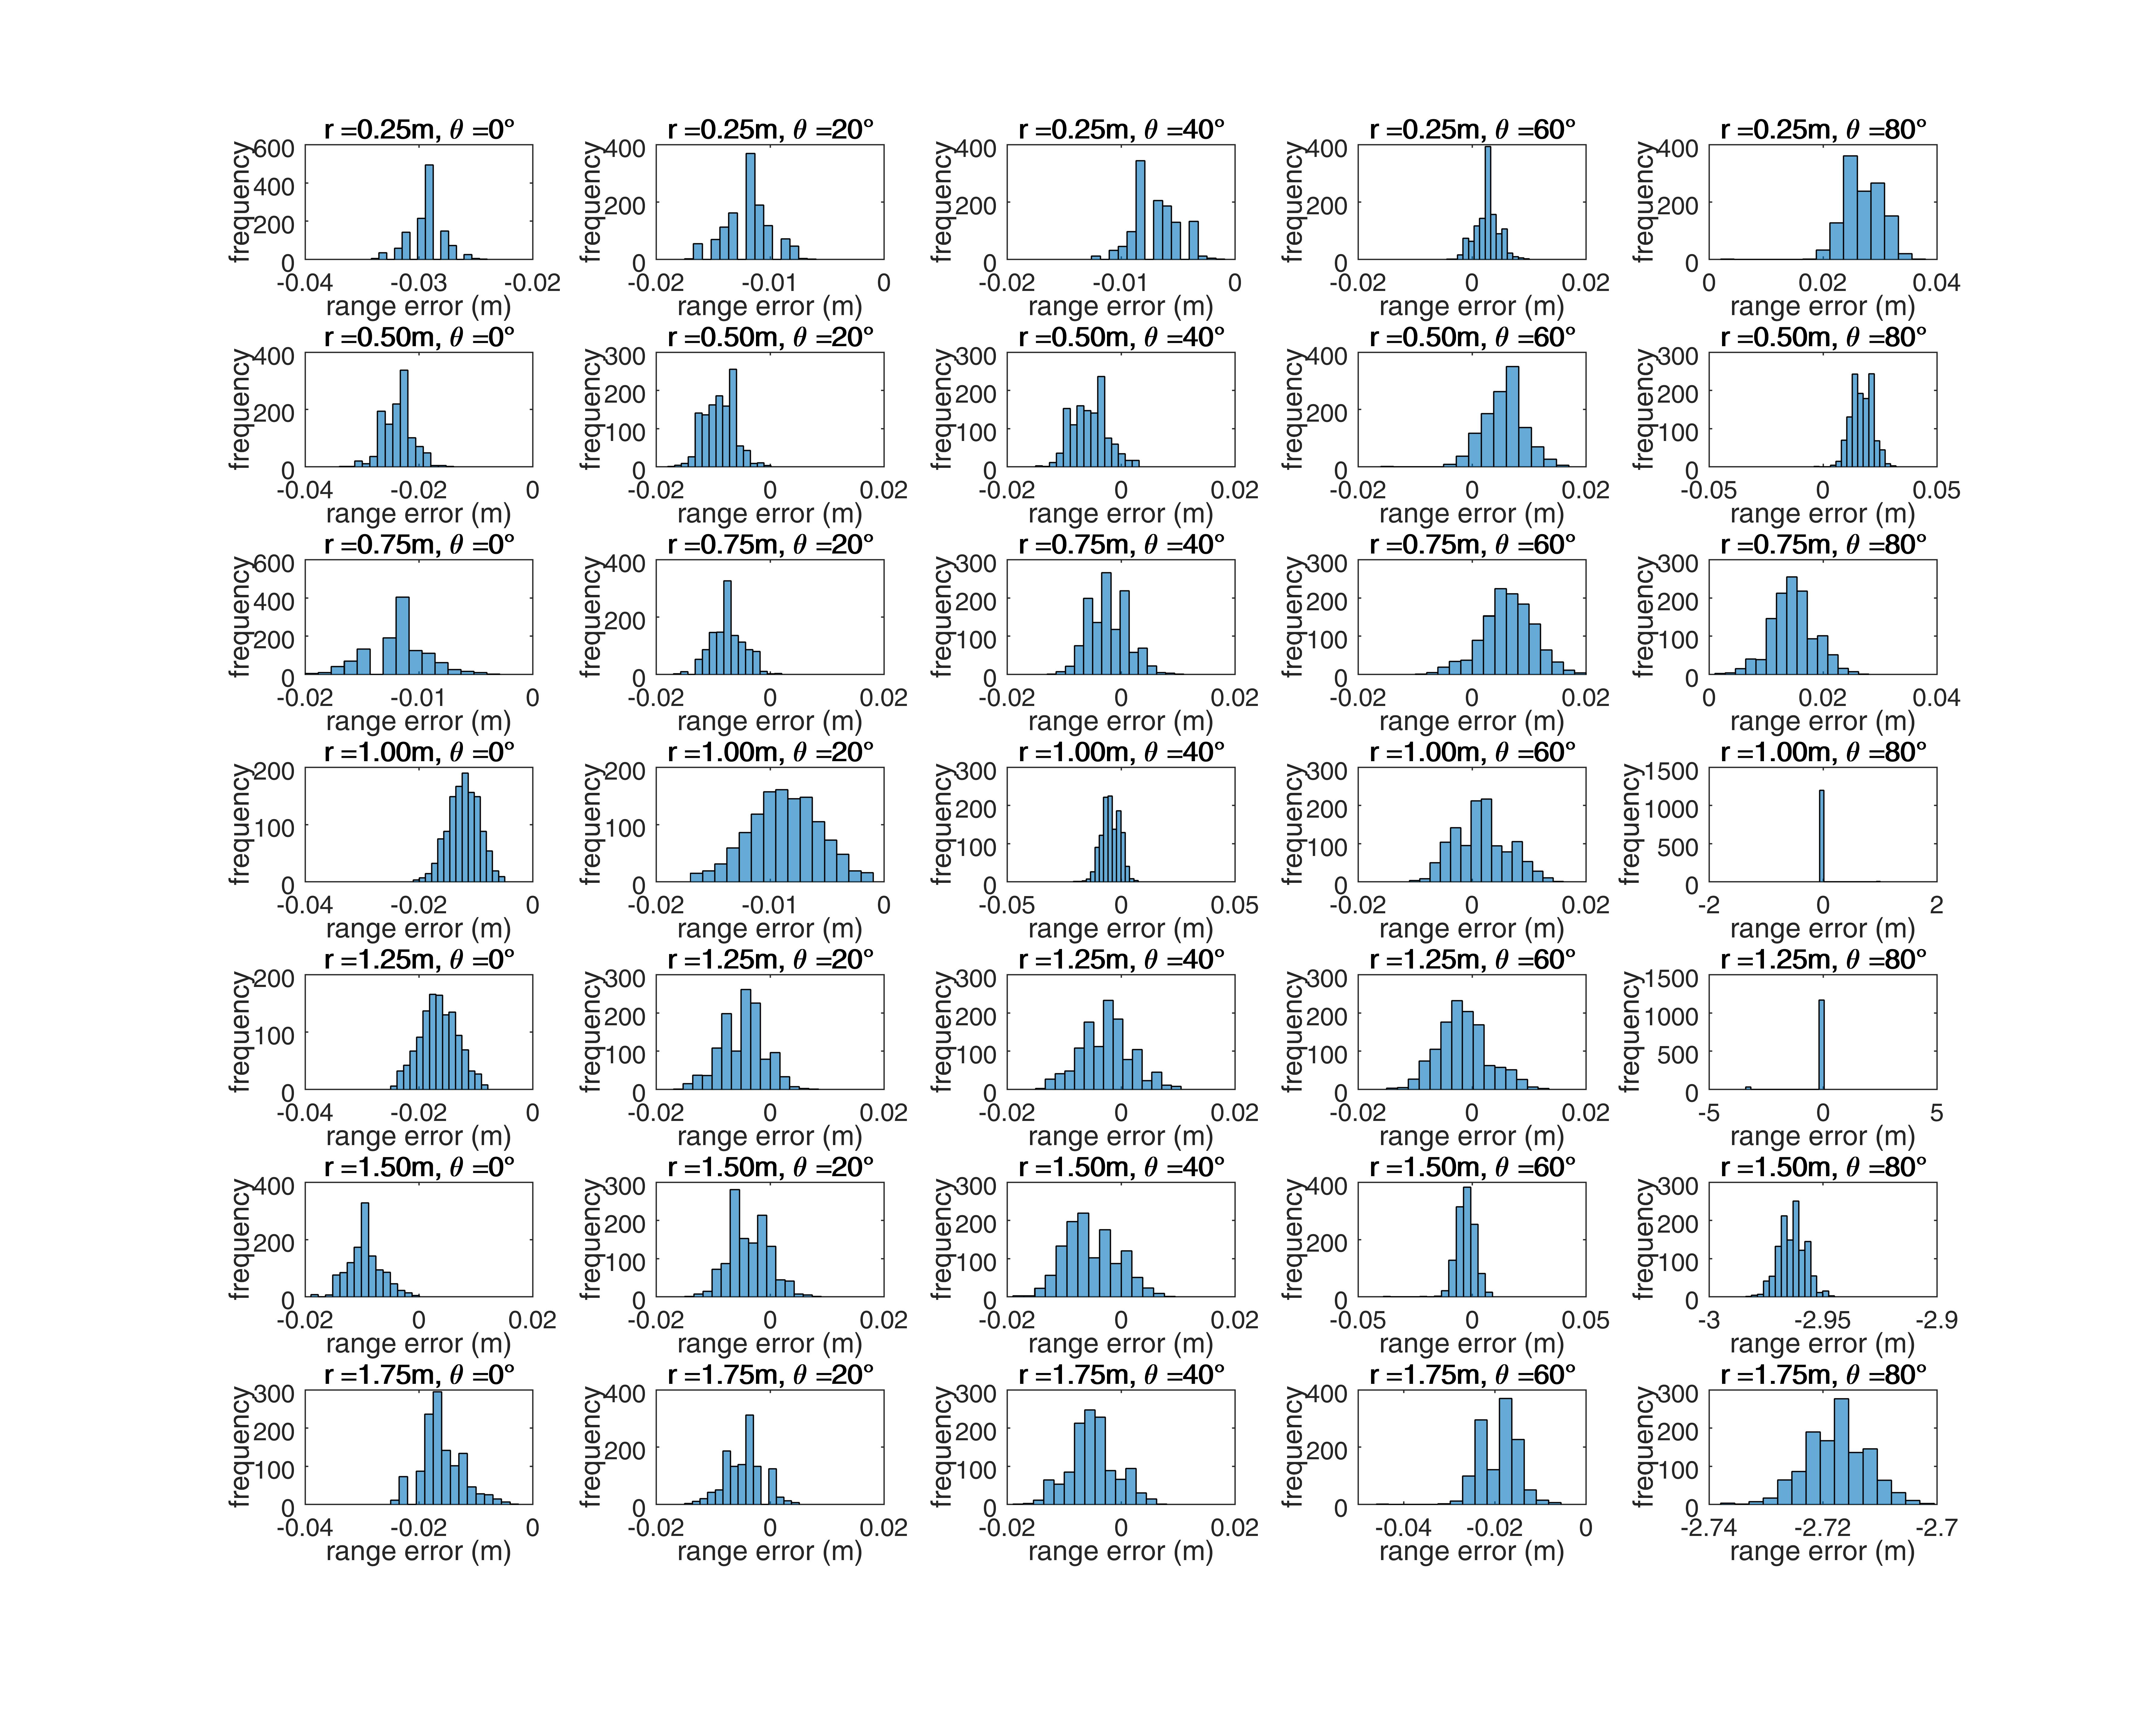
\includegraphics[width=1\textwidth,trim = 0mm 0mm 0mm 0mm,clip]{./Figures/range_error_histograms.jpg}
		  \caption{$r_{error}(r,\theta)$ approximately normally distributed}
		  \label{fig:mean_hist}
		\end{figure}
		
		Mean range error as function of (range,incidence angle) - Figure \ref{fig:mean_range_error}
		\begin{figure}
	  		\centering
	  		\subfigure[\label{fig:mean_range_error_outliers}]{
	  		\begin{minipage}[b]{0.45\columnwidth}
    			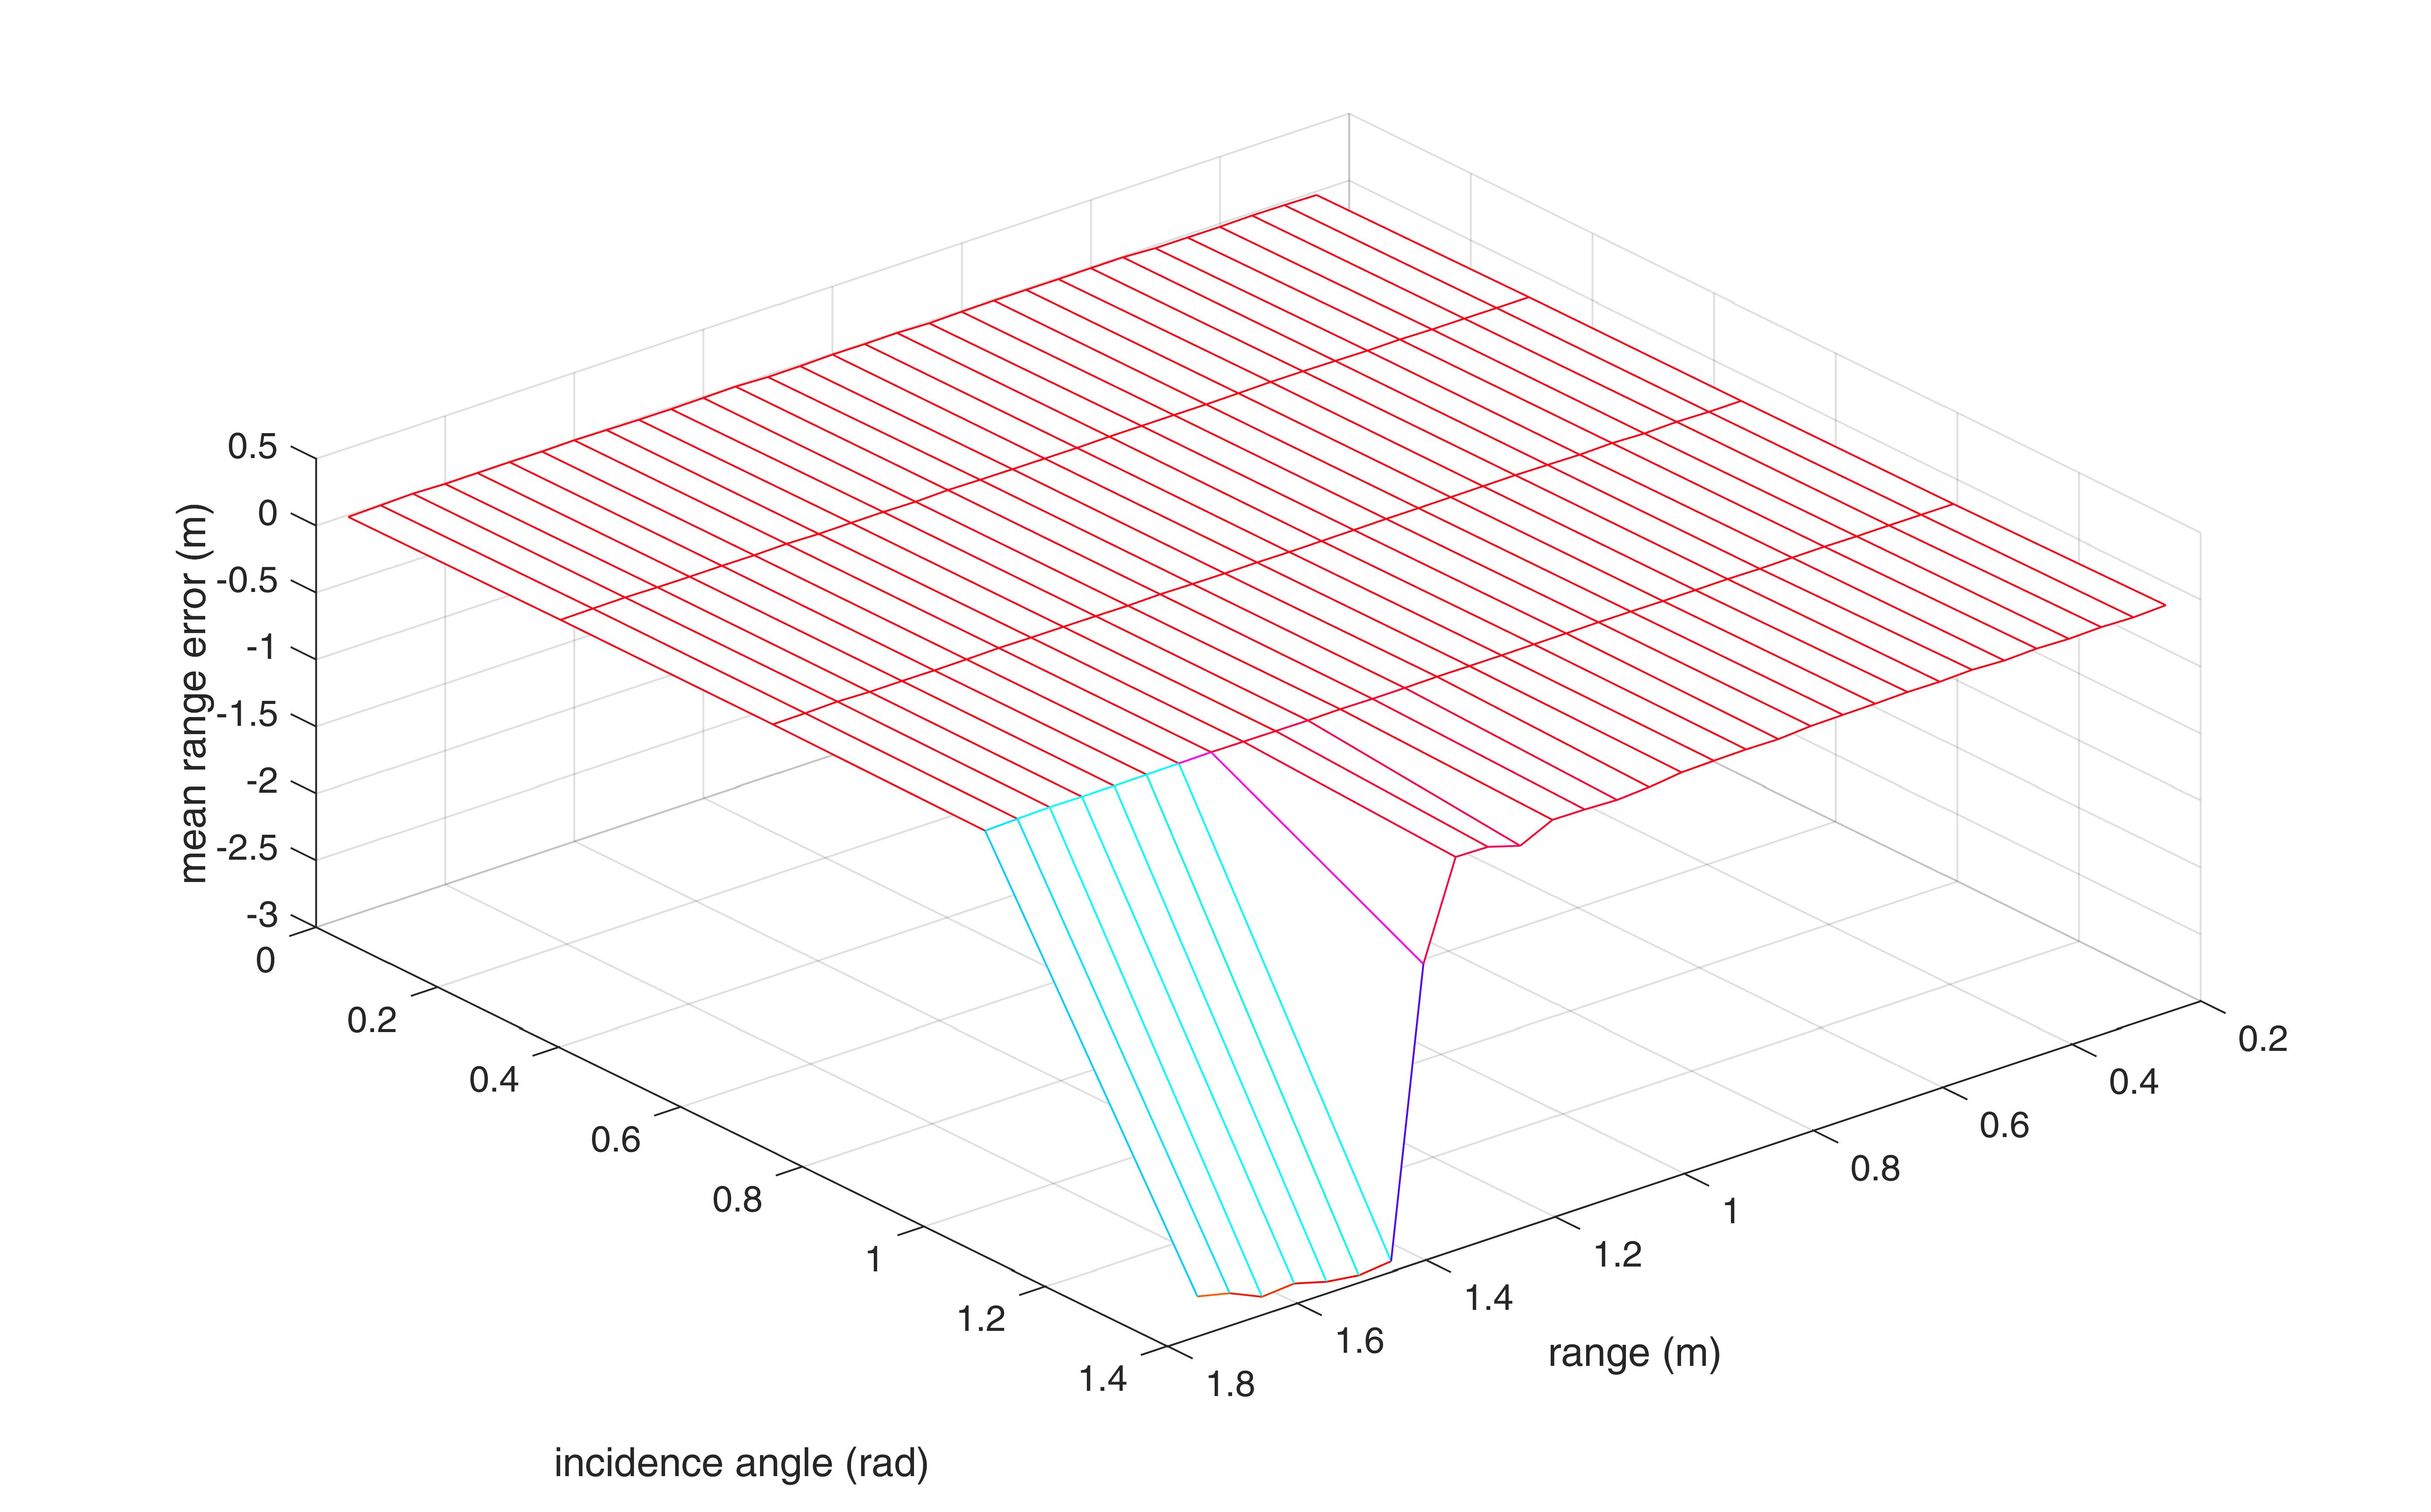
\includegraphics[width=1\textwidth,trim = 0mm 0mm 0mm 0mm,clip]{./Figures/noise_mean_range_error}\vspace*{0ex}
	  		\end{minipage}}
	  		\subfigure[\label{fig:mean_range_error_no_outliers}]{
	  		\begin{minipage}[b]{0.45\columnwidth}
    			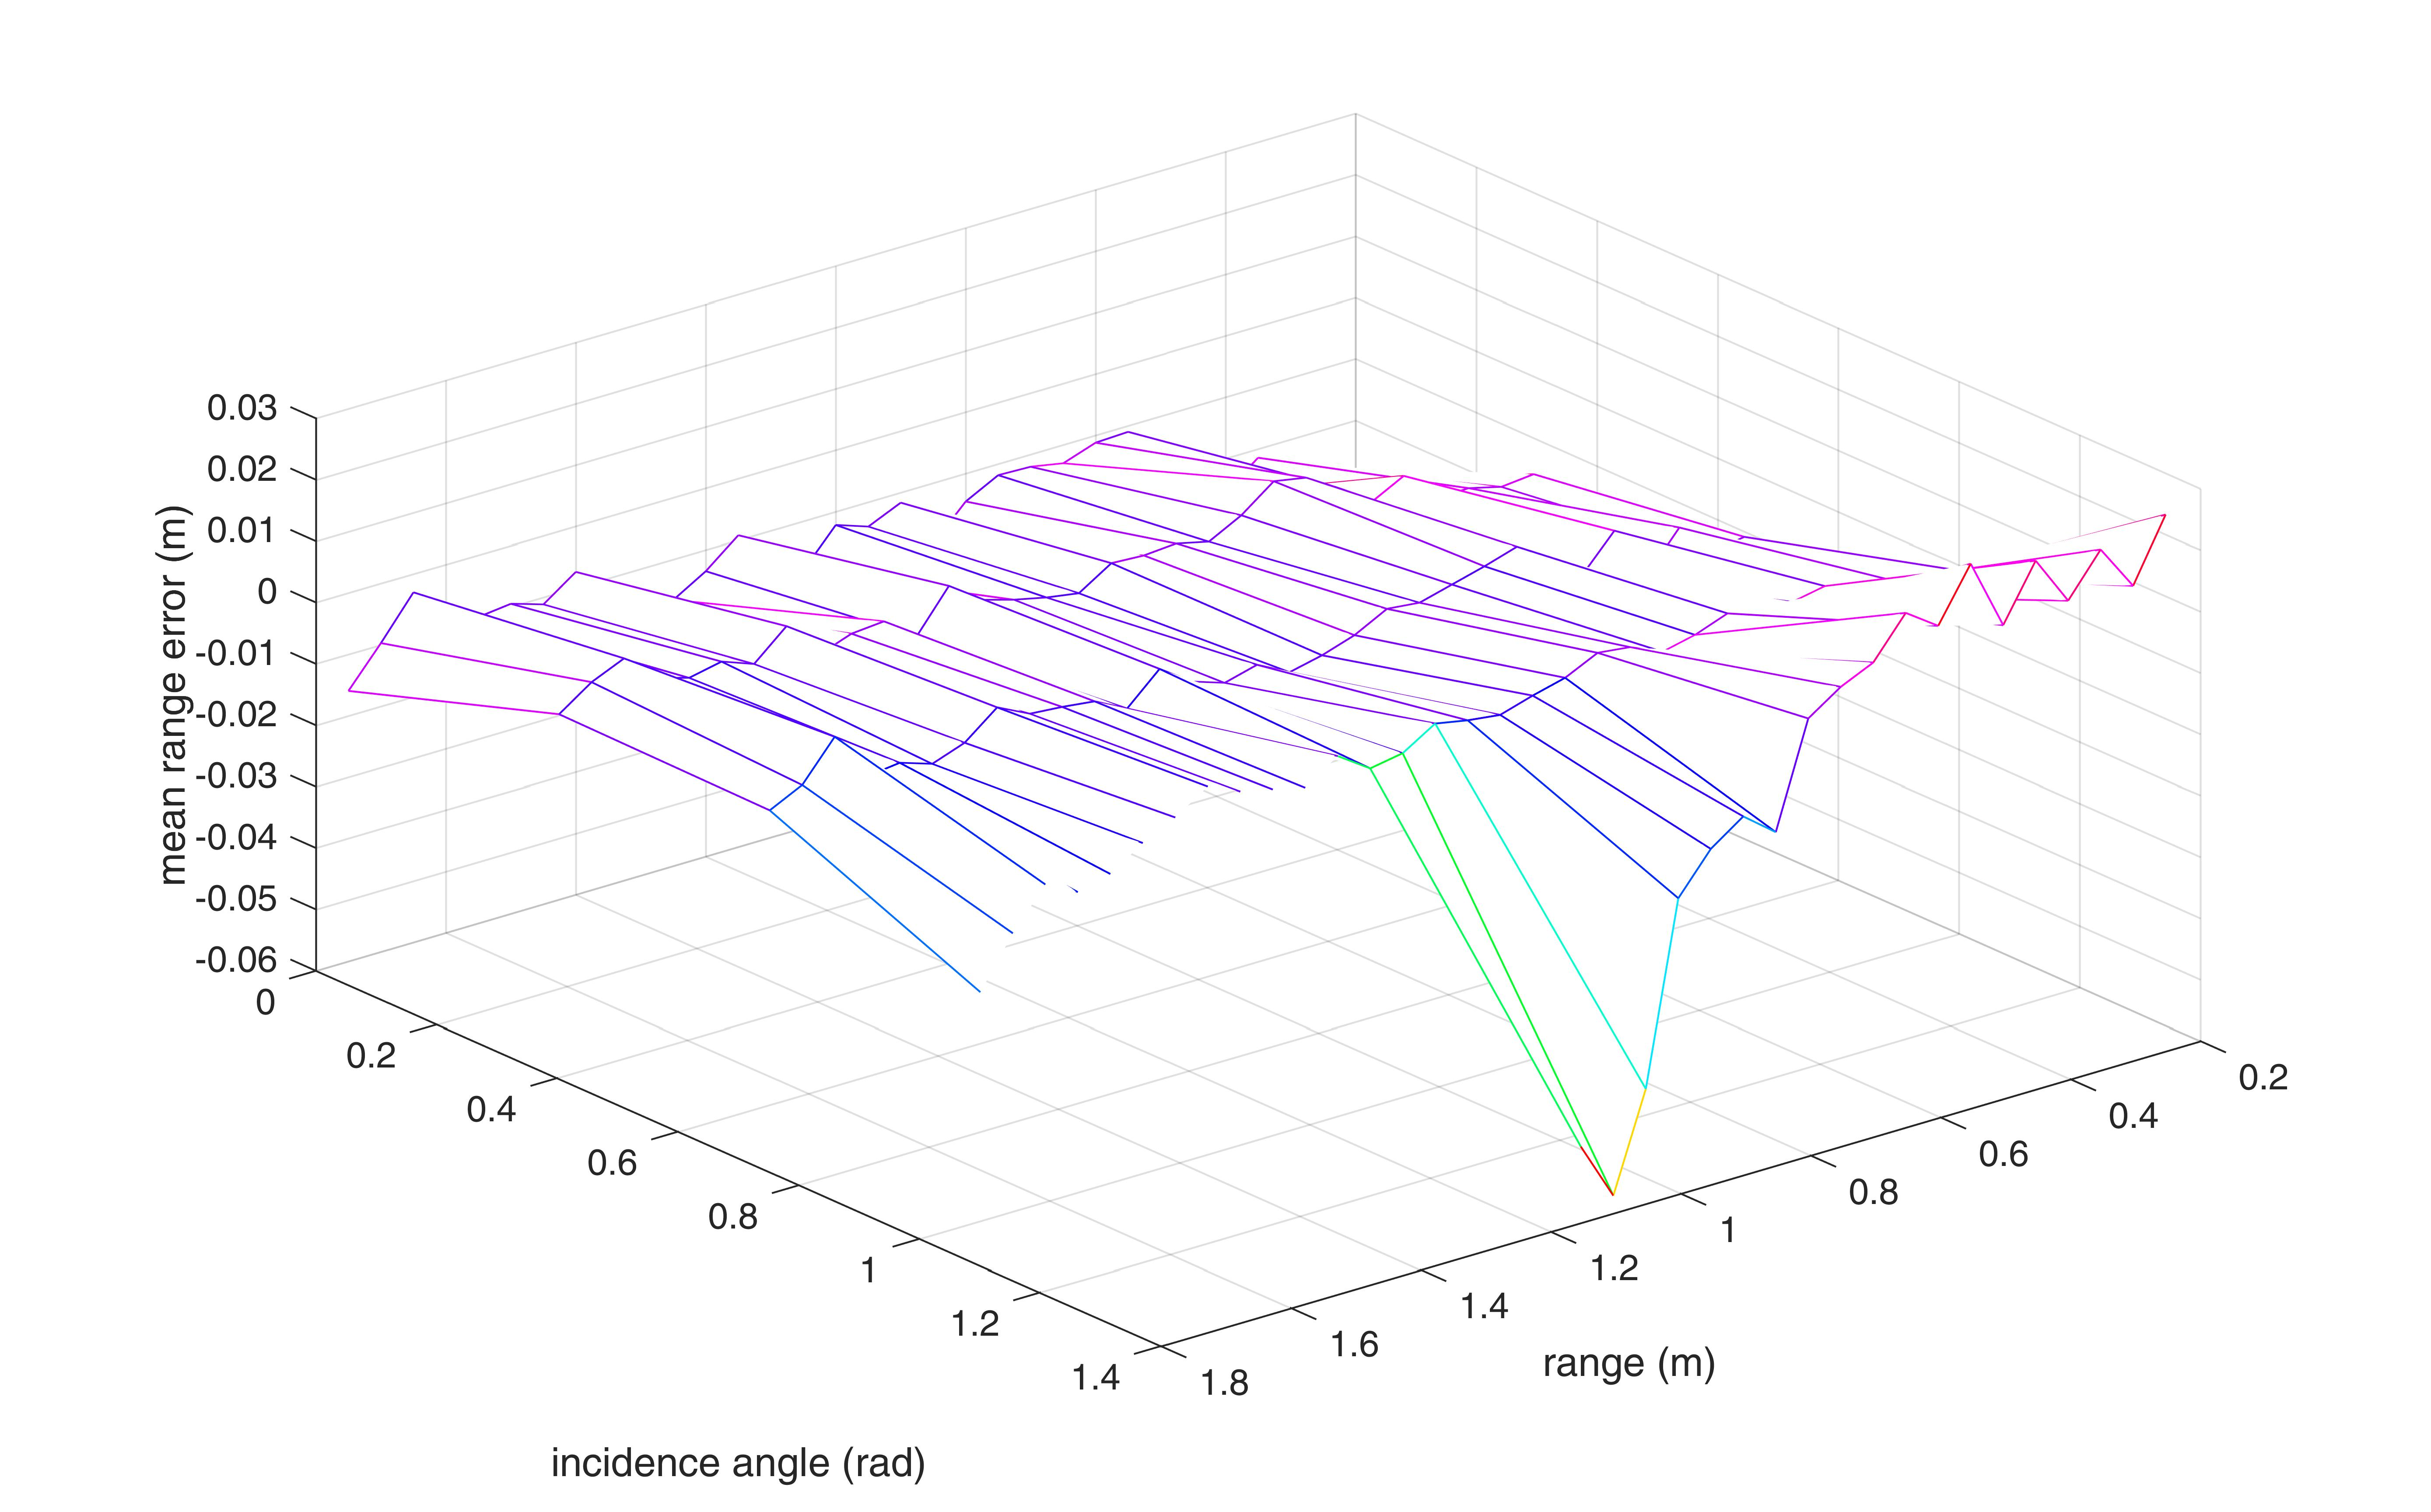
\includegraphics[width=1\textwidth,trim = 0mm 0mm 0mm 0mm,clip]{./Figures/noise_mean_range_error_removed_outliers}\vspace*{0ex}
		 \end{minipage}}
	  		\caption{mean range error vs $(r,\theta)$. (a) large error at high angles and range, (b) overall shape}
	  		\label{fig:mean_range_error}
		\end{figure}
		
		Std dev range error as function of (range,incidence angle) - Figure \ref{fig:stddev_range_error}		
		\begin{figure}
	  		\centering
	  		\subfigure[\label{fig:stddev_range_error_outliers}]{
	  		\begin{minipage}[b]{0.45\columnwidth}
    			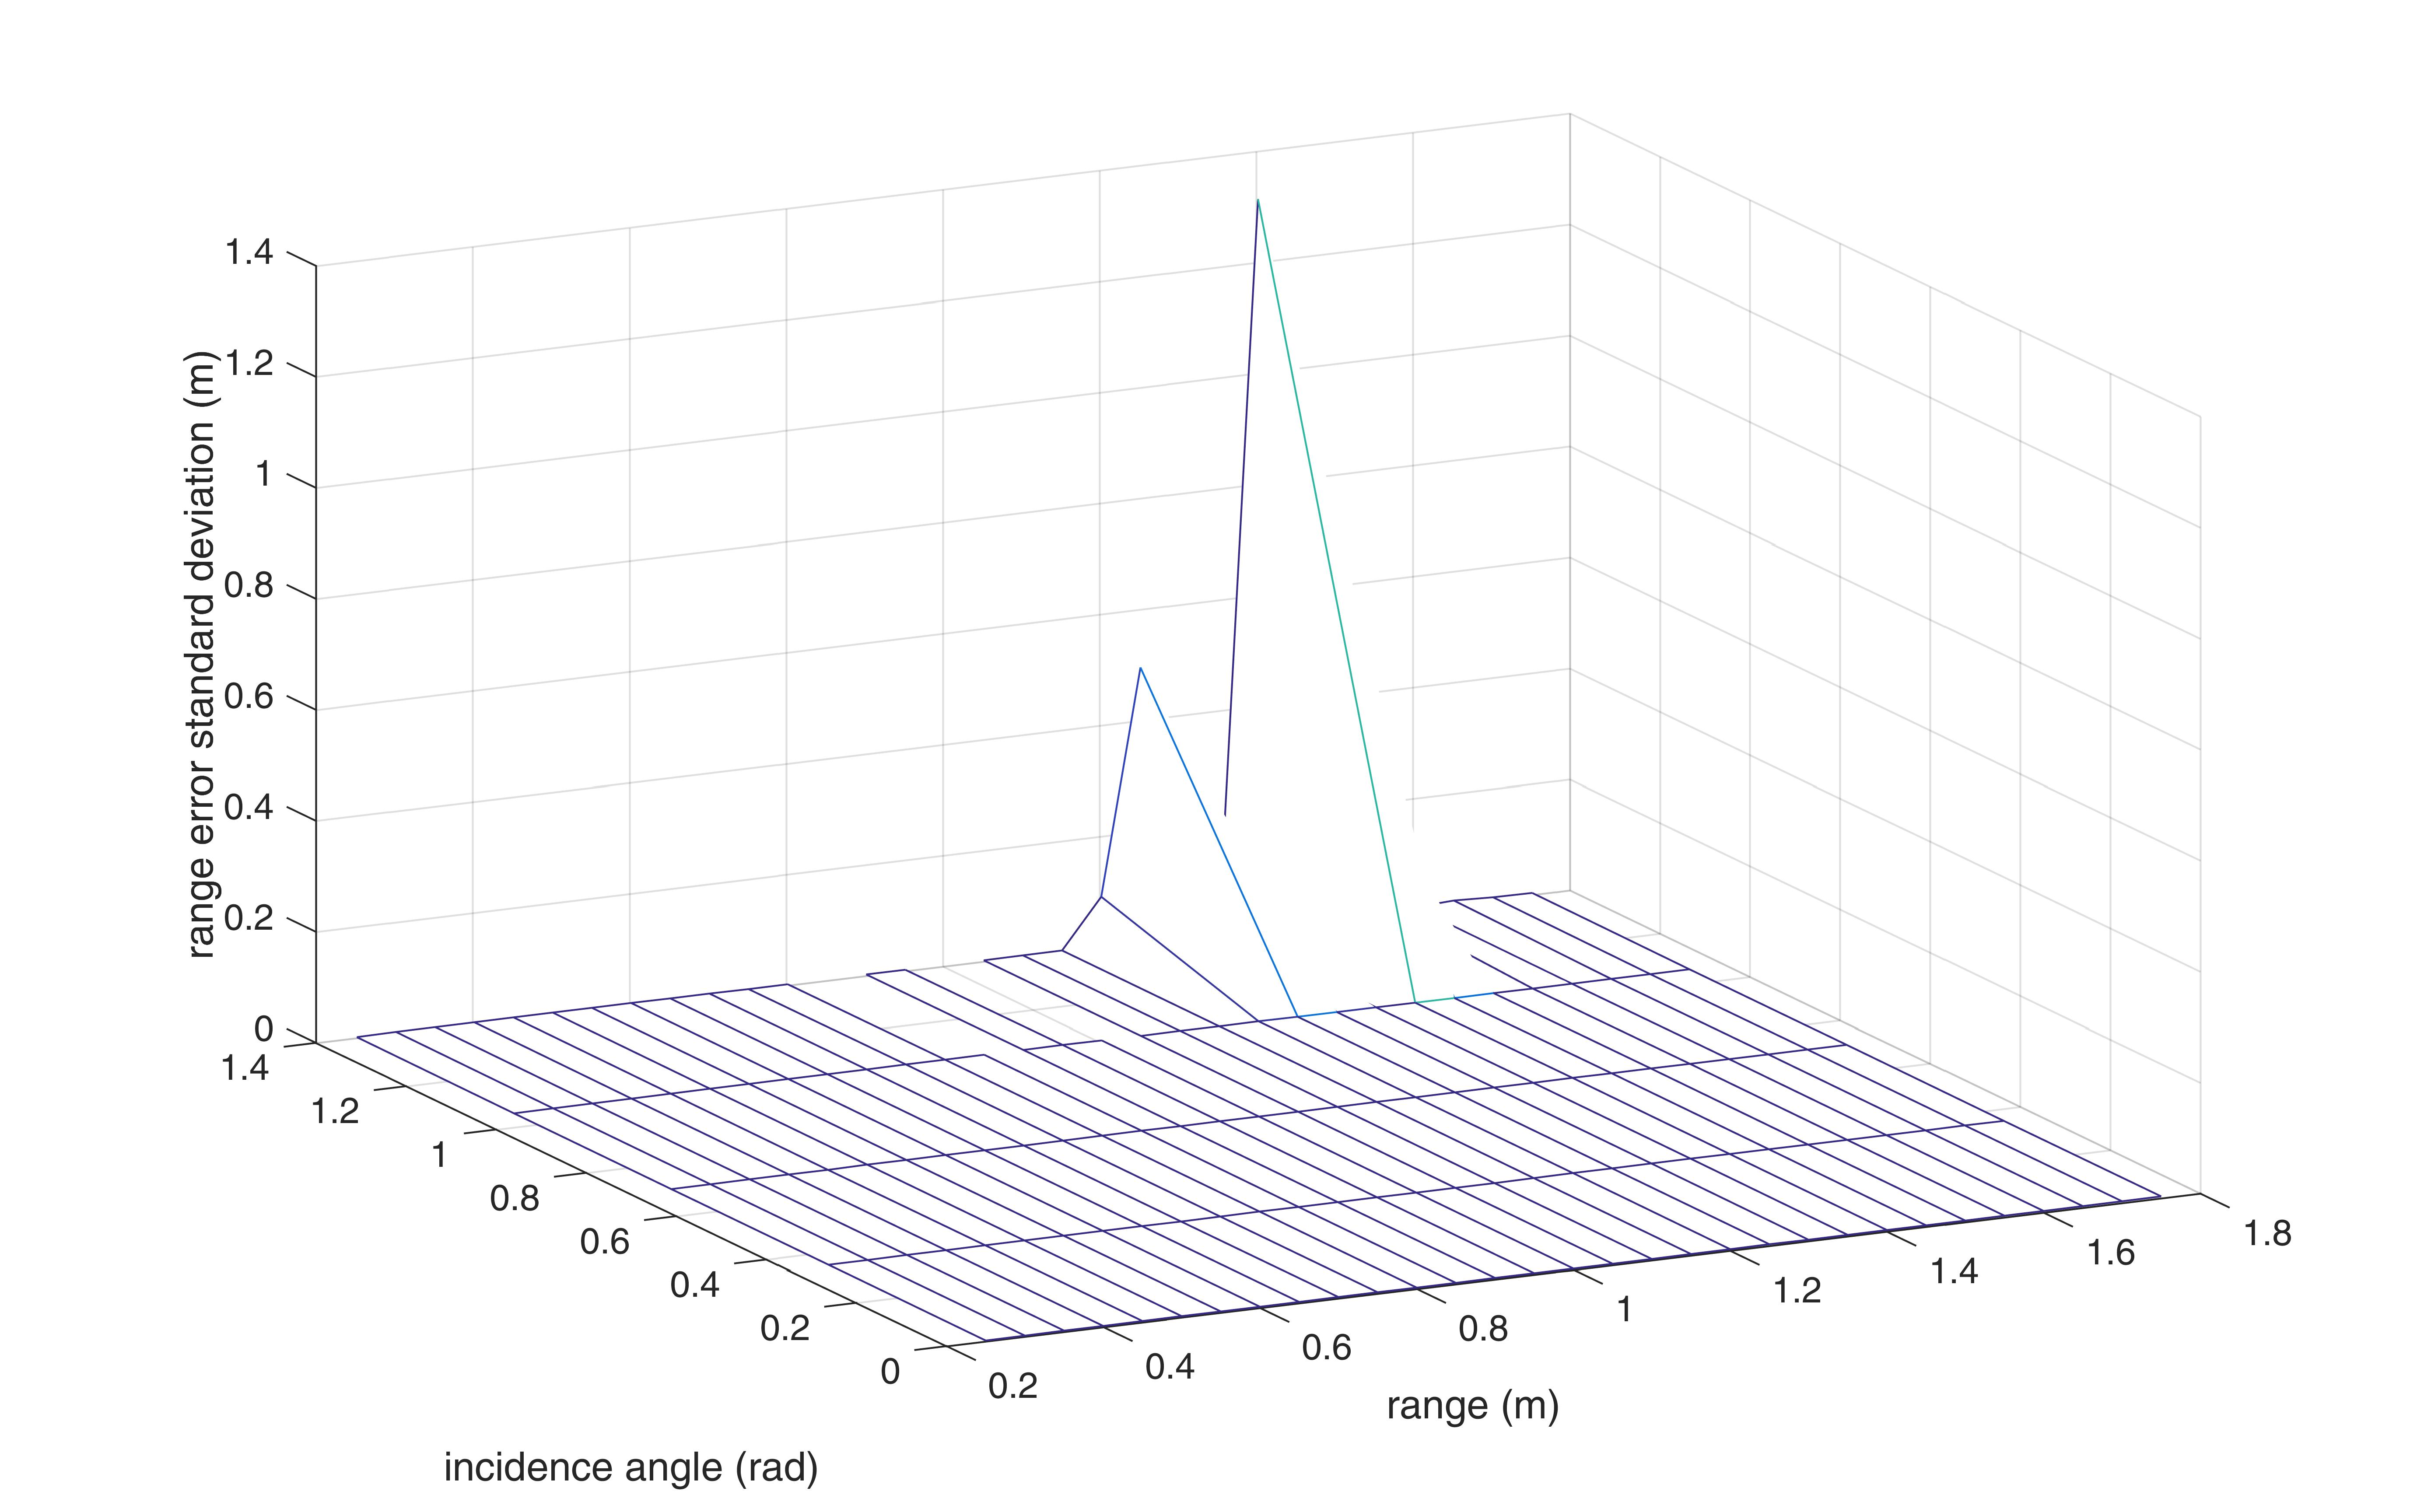
\includegraphics[width=1\textwidth,trim = 0mm 0mm 0mm 0mm,clip]{./Figures/noise_stddev_range_error}\vspace*{0ex}
	  		\end{minipage}}
	  		\subfigure[\label{fig:stddev_range_error_no_outliers}]{
	  		\begin{minipage}[b]{0.45\columnwidth}
    			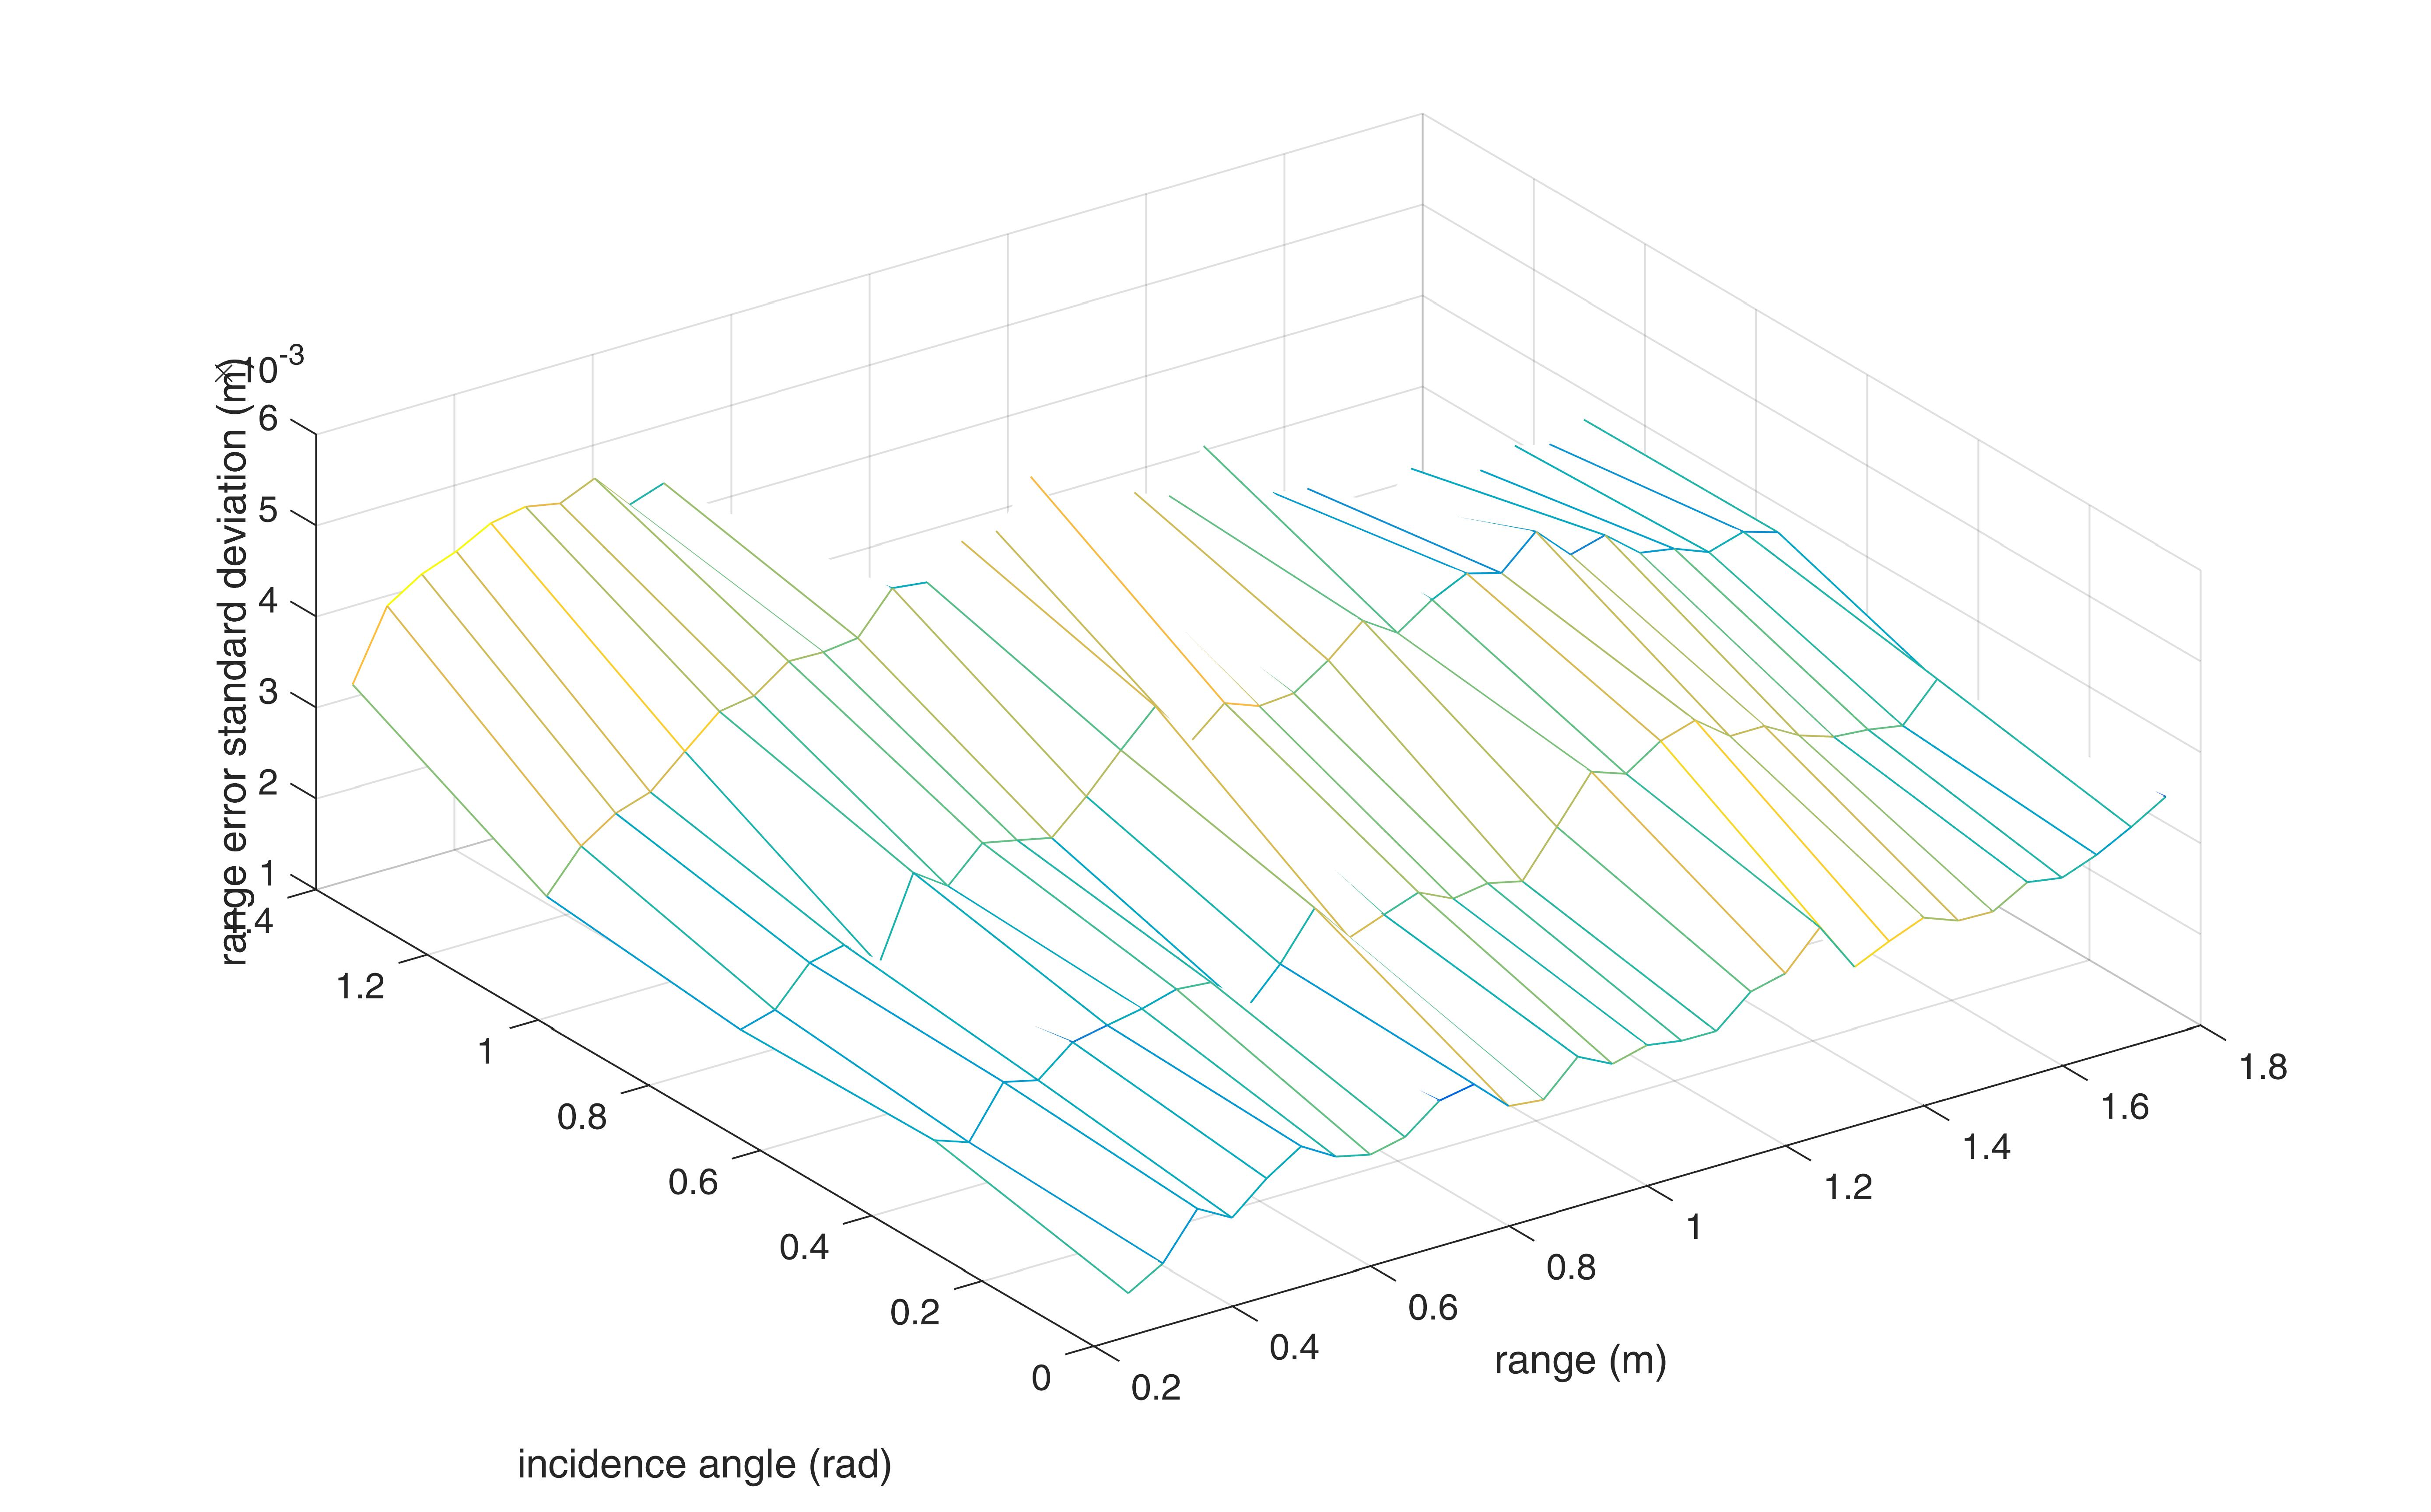
\includegraphics[width=1\textwidth,trim = 0mm 0mm 0mm 0mm,clip]{./Figures/noise_stddev_range_error_removed_outliers}\vspace*{0ex}
	 		 \end{minipage}}
	  		\caption{range error $\sigma$ vs $(r,\theta)$. (a) outliers/large std dev at high angles and range, (b) overall shape}
	  		\label{fig:stddev_range_error}
		\end{figure}
		
		Fitted 4th degree (in $x$ and $y$) polynomials to data points - Figure \ref{fig:surface_range_error}. INCLUDE FIT DATA
		\begin{figure}
	  		\centering
	  		\subfigure[\label{fig:surface_mean_range}]{
	  		\begin{minipage}[b]{0.45\columnwidth}
    			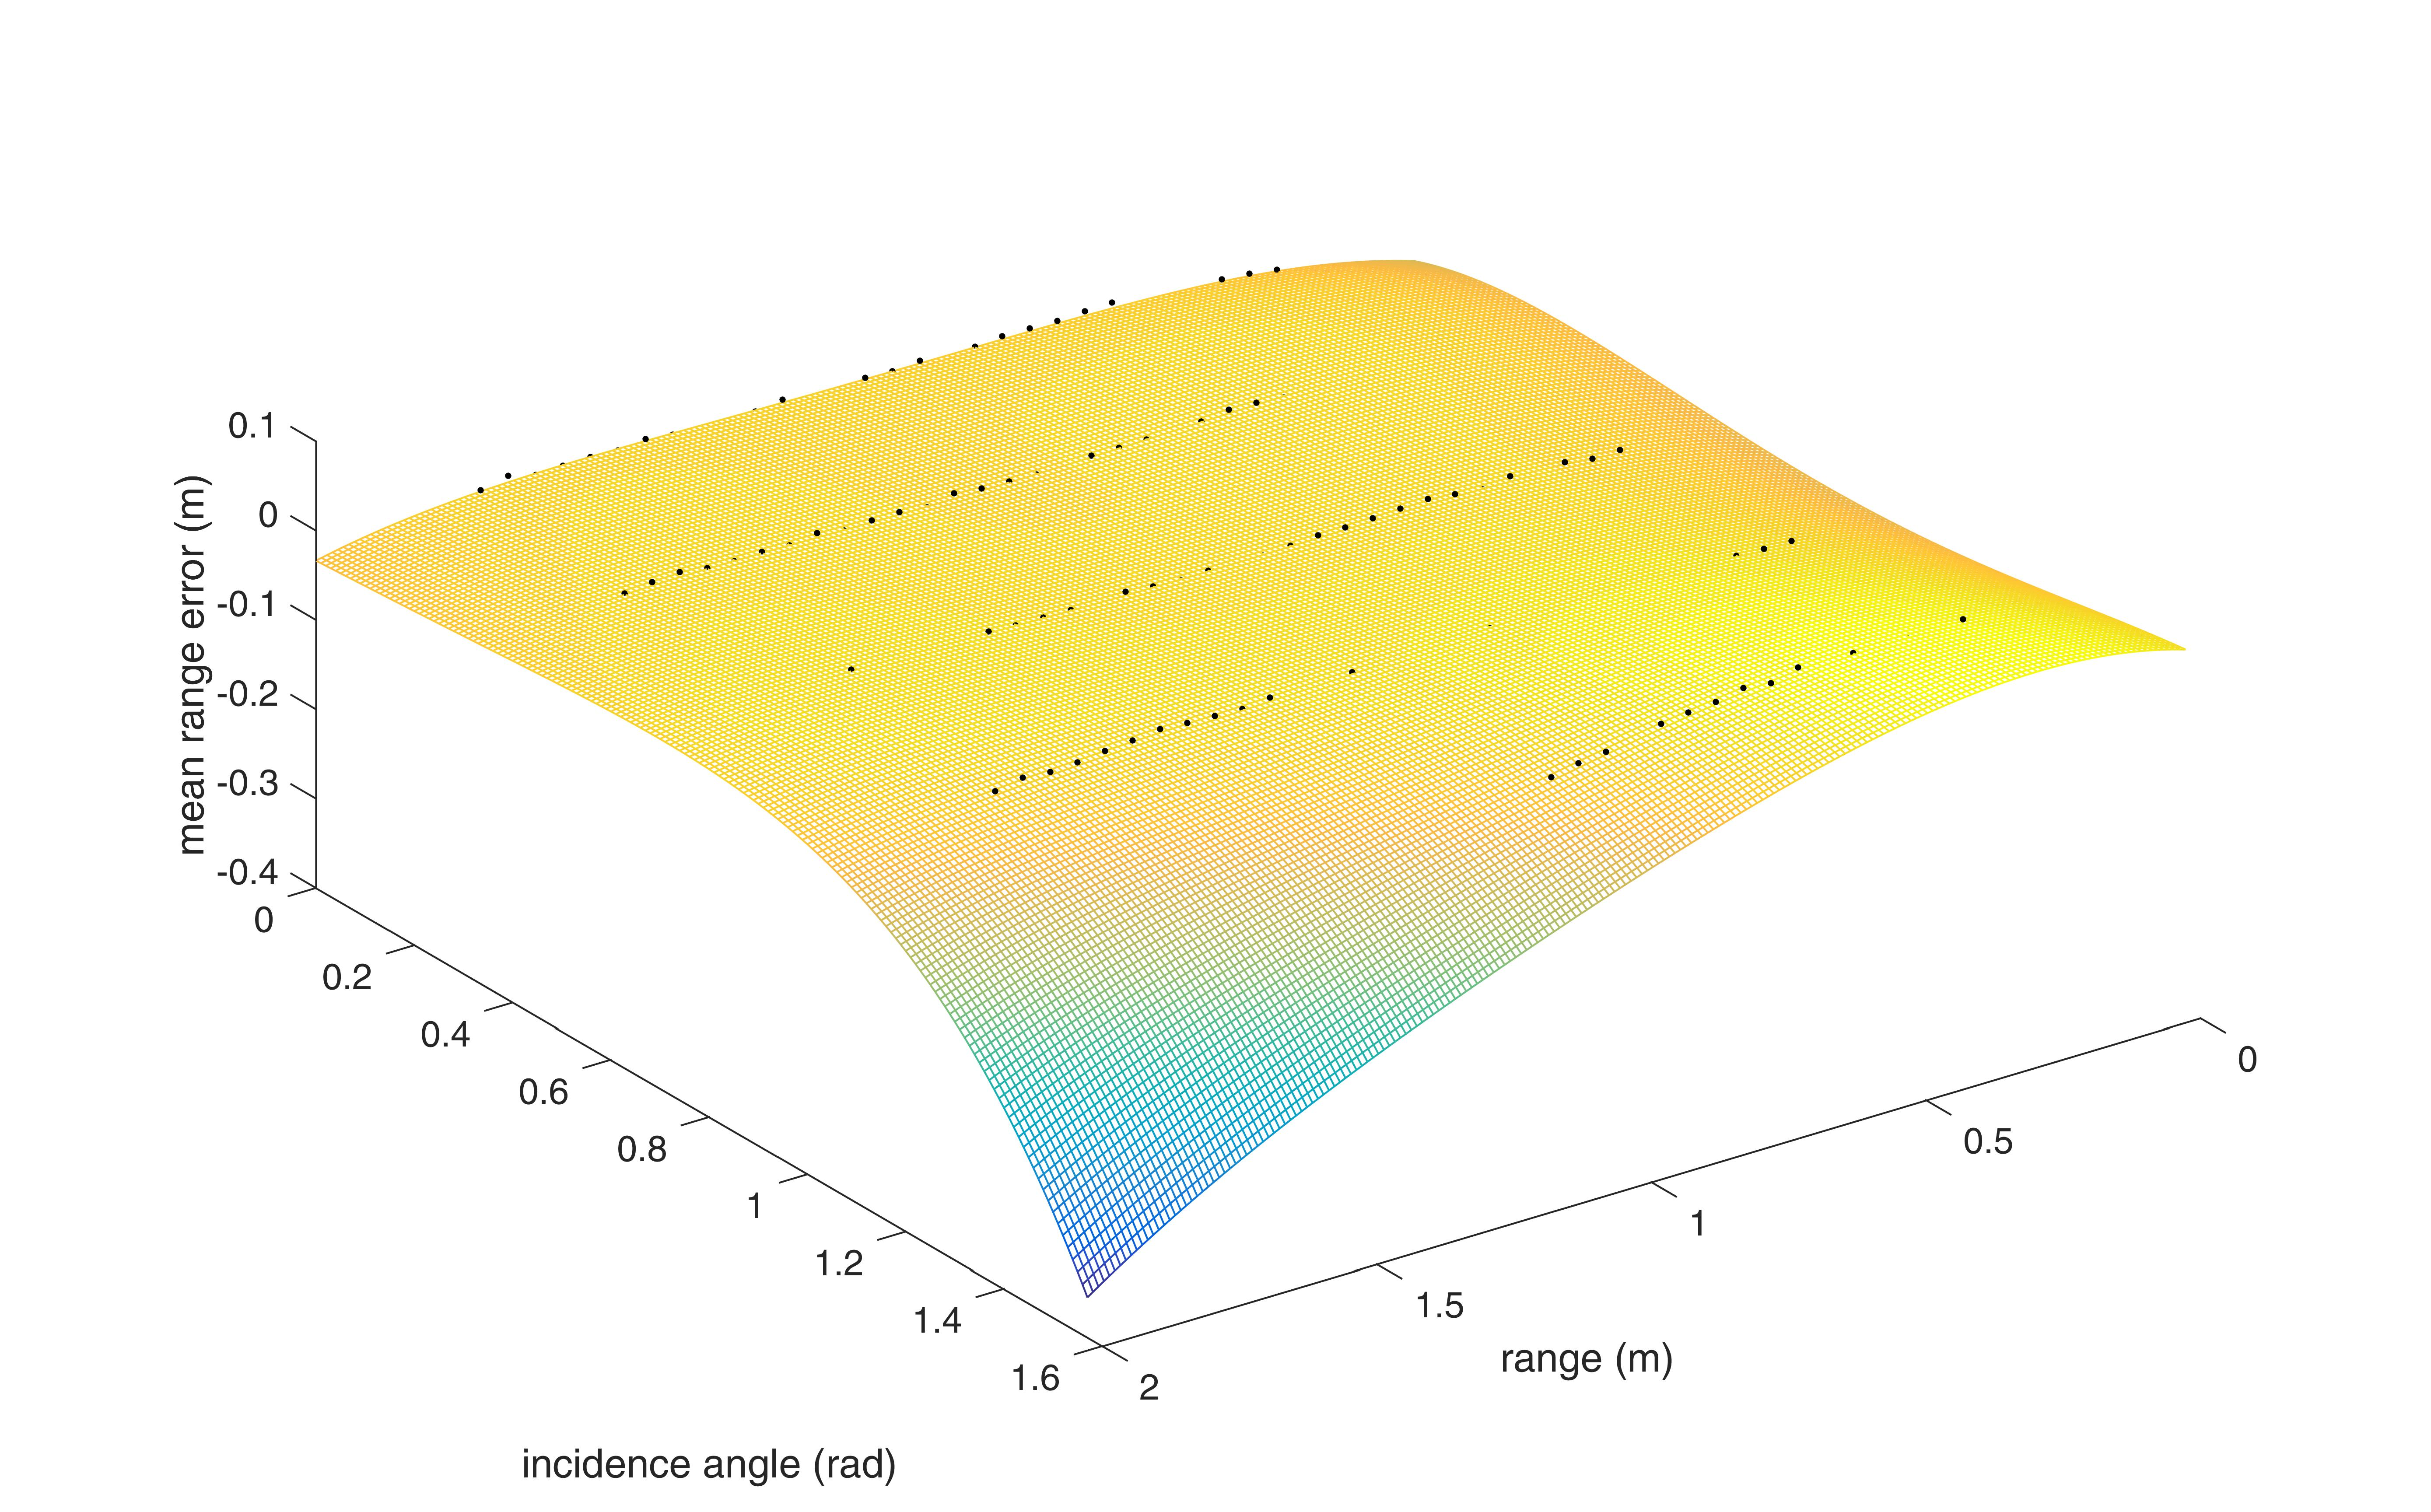
\includegraphics[width=1\textwidth,trim = 0mm 0mm 0mm 0mm,clip]{./Figures/surface_mean_range_error}\vspace*{0ex}
	  		\end{minipage}}
	  		\subfigure[\label{fig:surface_stddev_range}]{
	  		\begin{minipage}[b]{0.45\columnwidth}
    			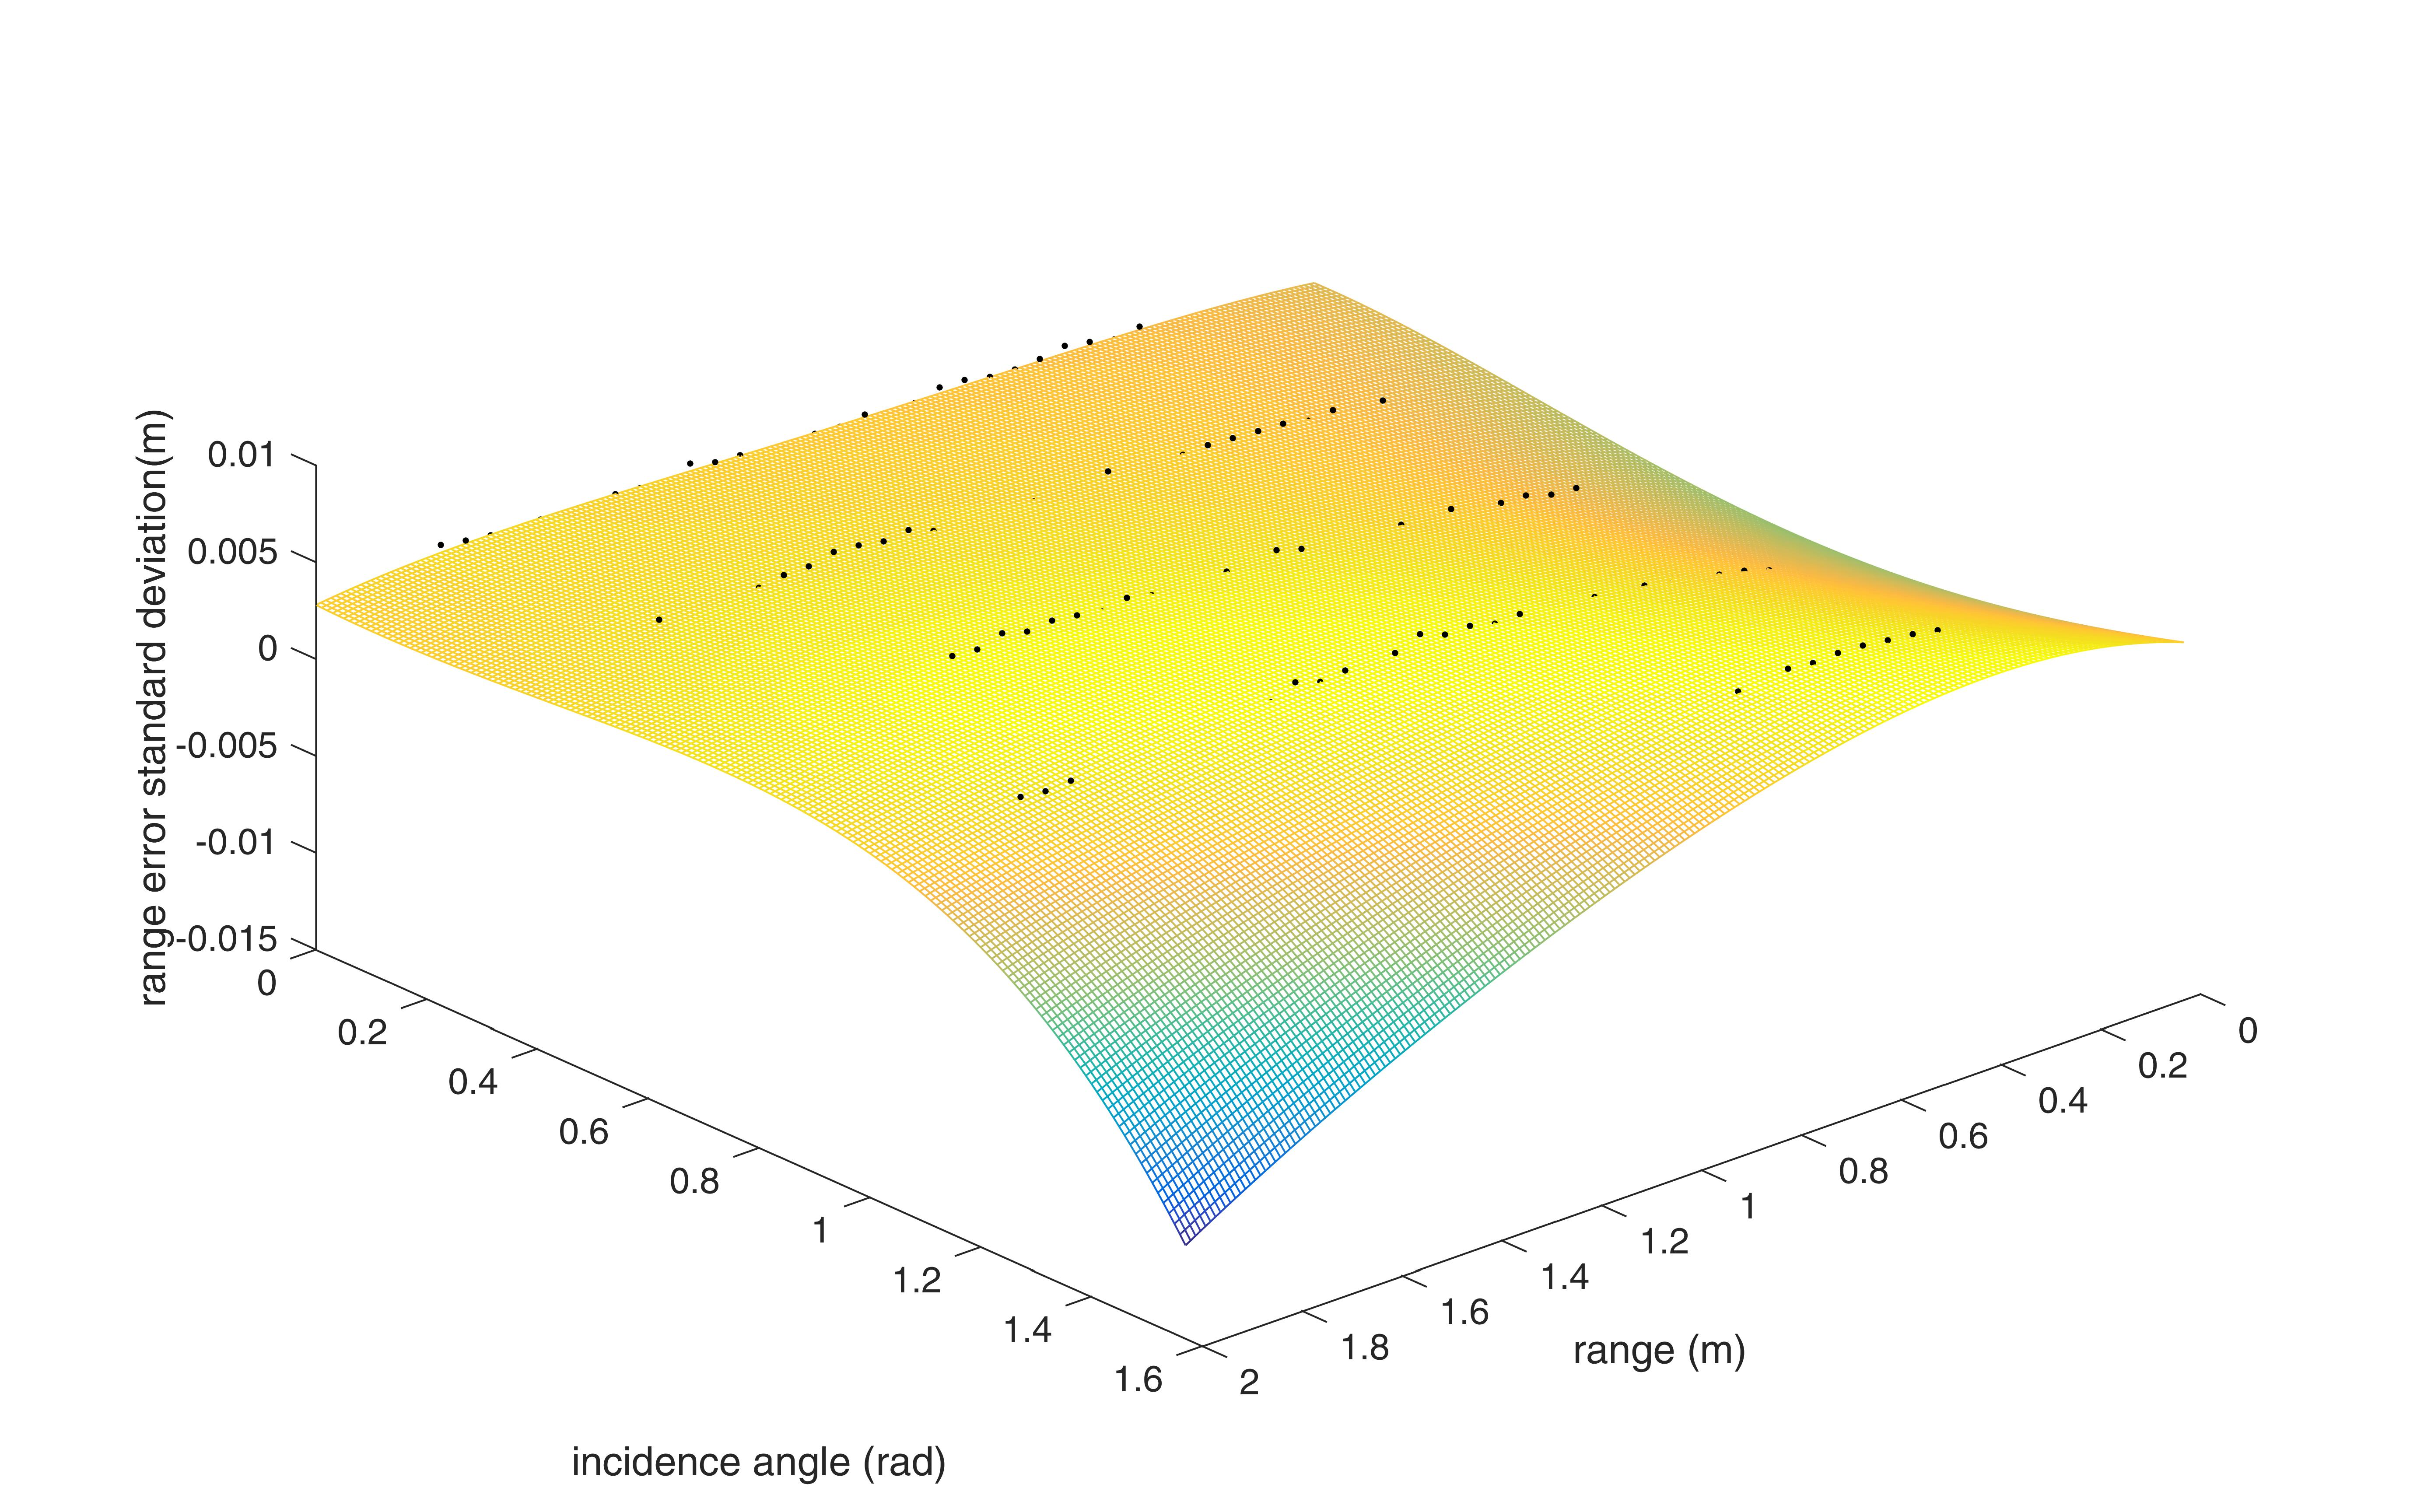
\includegraphics[width=1\textwidth,trim = 0mm 0mm 0mm 0mm,clip]{./Figures/surface_stddev_range_error}\vspace*{0ex}
		 \end{minipage}}
	  		\caption{polynomials fitted to range error mean \& standard deviation data points to model noise}
	  		\label{fig:surface_range_error}
		\end{figure}
		
		Noise Model:\\
		\begin{equation}
			\hat{r} = f_s(r,\theta,\phi(k)) = r + \mathcal{N}(\mu,\sigma)
		\end{equation}	
		
		\begin{equation}
			\begin{aligned}
				\mu = & a_{00} + a_{10}r + a_{01}\theta + a_{20}r^2 + a_{11}r\theta + a_{02}\theta^2\\
				      & + a_{30}r^3 + a_{21}r^2\theta + a_{12}r\theta^2 + a_{03}\theta^3 + a_{40}r^4 \\ 
				      & + a_{31}r^3\theta + a_{22}r^2\theta^2 + a_{13}r\theta^3 + a_{04}\theta^4
			\end{aligned}		
		\end{equation}
		\begin{equation}
			\begin{aligned}
				\sigma = & b_{00} + b_{10}r + b_{01}\theta + b_{20}r^2 + b_{11}r\theta + b_{02}\theta^2\\
			         	 & + b_{30}r^3 + b_{21}r^2\theta + b_{12}r\theta^2 + b_{03}\theta^3 + a_{40}r^4 \\ 
			         	 & + b_{31}r^3\theta + b_{22}r^2\theta^2 + b_{13}r\theta^3 + b_{04}\theta^4
			\end{aligned}
		\end{equation}
		
		*outliers ignored in model. if angle $>$ 75 deg and range $>$ 0.8m, range measurement = NaN. EXPLANATION: as angle increases, measured range becomes less than ground truth - due to beam width. part of beam hits part of object that is closer due to angle. However, as angle increases further, not enough light returns to make measurements. At high ranges and angles, measurement is not of object, but due to reflections that take much longer. Measurement ends up being near maximum range or even INF. Instead, will set as NaN - no value returned.
		
		Coefficients in tables \ref{tab:noise_a} and \ref{tab:noise_b}
		\begin{table}[h!]
  \centering
  \caption{$a_{ij}$ coefficients}
  \label{tab:noise_a}
  \begin{tabular}{c| c c c c c}
     	  & $j_0$ 	 & $j_1$   & $j_2$ 	 & $j_3$   & $j_4$ \\
    \hline
   	$i_0$ & -0.06529 & 0.2126  & -0.533	 & 0.4629  & -0.1223 \\
   	$i_1$ & 0.2024   & -0.1906 & 0.4006	 & -0.1791 & 0 \\
   	$i_2$ & -0.3074  & 0.0228  & -0.0716 & 0 	   & 0 \\
   	$i_3$ & 0.2053   & 0.01455 & 0 		 & 0 	   & 0 \\
   	$i_4$ & -0.04912 & 0 	   & 0 		 & 0 	   & 0 \\
  \end{tabular}
\end{table}



		\begin{table}[h!]
  \centering
  \caption{$b_{ij}$ coefficients}
  \label{tab:noise_b}
  \begin{tabular}{c| c c c c c}
		  & $j_0$ 	  & $j_1$    & $j_2$ 	  & $j_3$	  & $j_4$ \\
	\hline
	$i_0$ & 0.001242  & 0.2126	 & -0.01128	  & 0.01162	  & -0.002746 \\
	$i_1$ & 0.00352   & 0.006146 & 0.01021	  & -0.007316 & 0 \\
	$i_2$ & -0.005138 & -0.00626 & -0.0005068 & 0 		  & 0 \\
	$i_3$ & 0.004067  & 0.001337 & 0 		  & 0 		  & 0 \\
	$i_4$ & -0.001092 & 0 		 & 0 		  & 0 		  & 0 \\
  \end{tabular}
\end{table}





		\textbf{Surface noise:}
		random walk model\\
		have observed error mostly independent of range and angle - seems to be some compensation performed by sensor to get straight lines - range across smooth surfaces that should be appear as straight lines varies regularly.
		Could be surface properties of objects, though error is larger than expected in this case.
		Profile of error sinusoidal (regular-ish peaks and valleys), peaks = 5mm deep \& 50mm wide approximately
		
		add random walk to each scan
		\begin{equation}
			error = a\sum_{n = 1}^{n_{Steps}}-1 + 2\:\left \lfloor{\mathcal{R}}\right \rfloor 
		\end{equation} 
		where $\mathcal{R}$ is a random variable following a uniform distribution on [0,1]. Chose step size of $a = 0.0005m$
		Doesn't work too well over long surfaces (~1m) - can get too large sometimes, but fits measured data for small objects like cube
		
		Figure \ref{fig:surface_noise}: comparison of simulated \& measured surface noise:
		\textbf{ERROR BARS INSTEAD OF DOTS}. MENTION THAT IT IS FLIPPED, COULD BE OTHER WAY. DUE TO RANDOM WALK.
		\begin{figure}
	  		\centering
	  		\subfigure[\label{fig:measured_surface_noise}]{
	  		\begin{minipage}[b]{0.45\columnwidth}
    			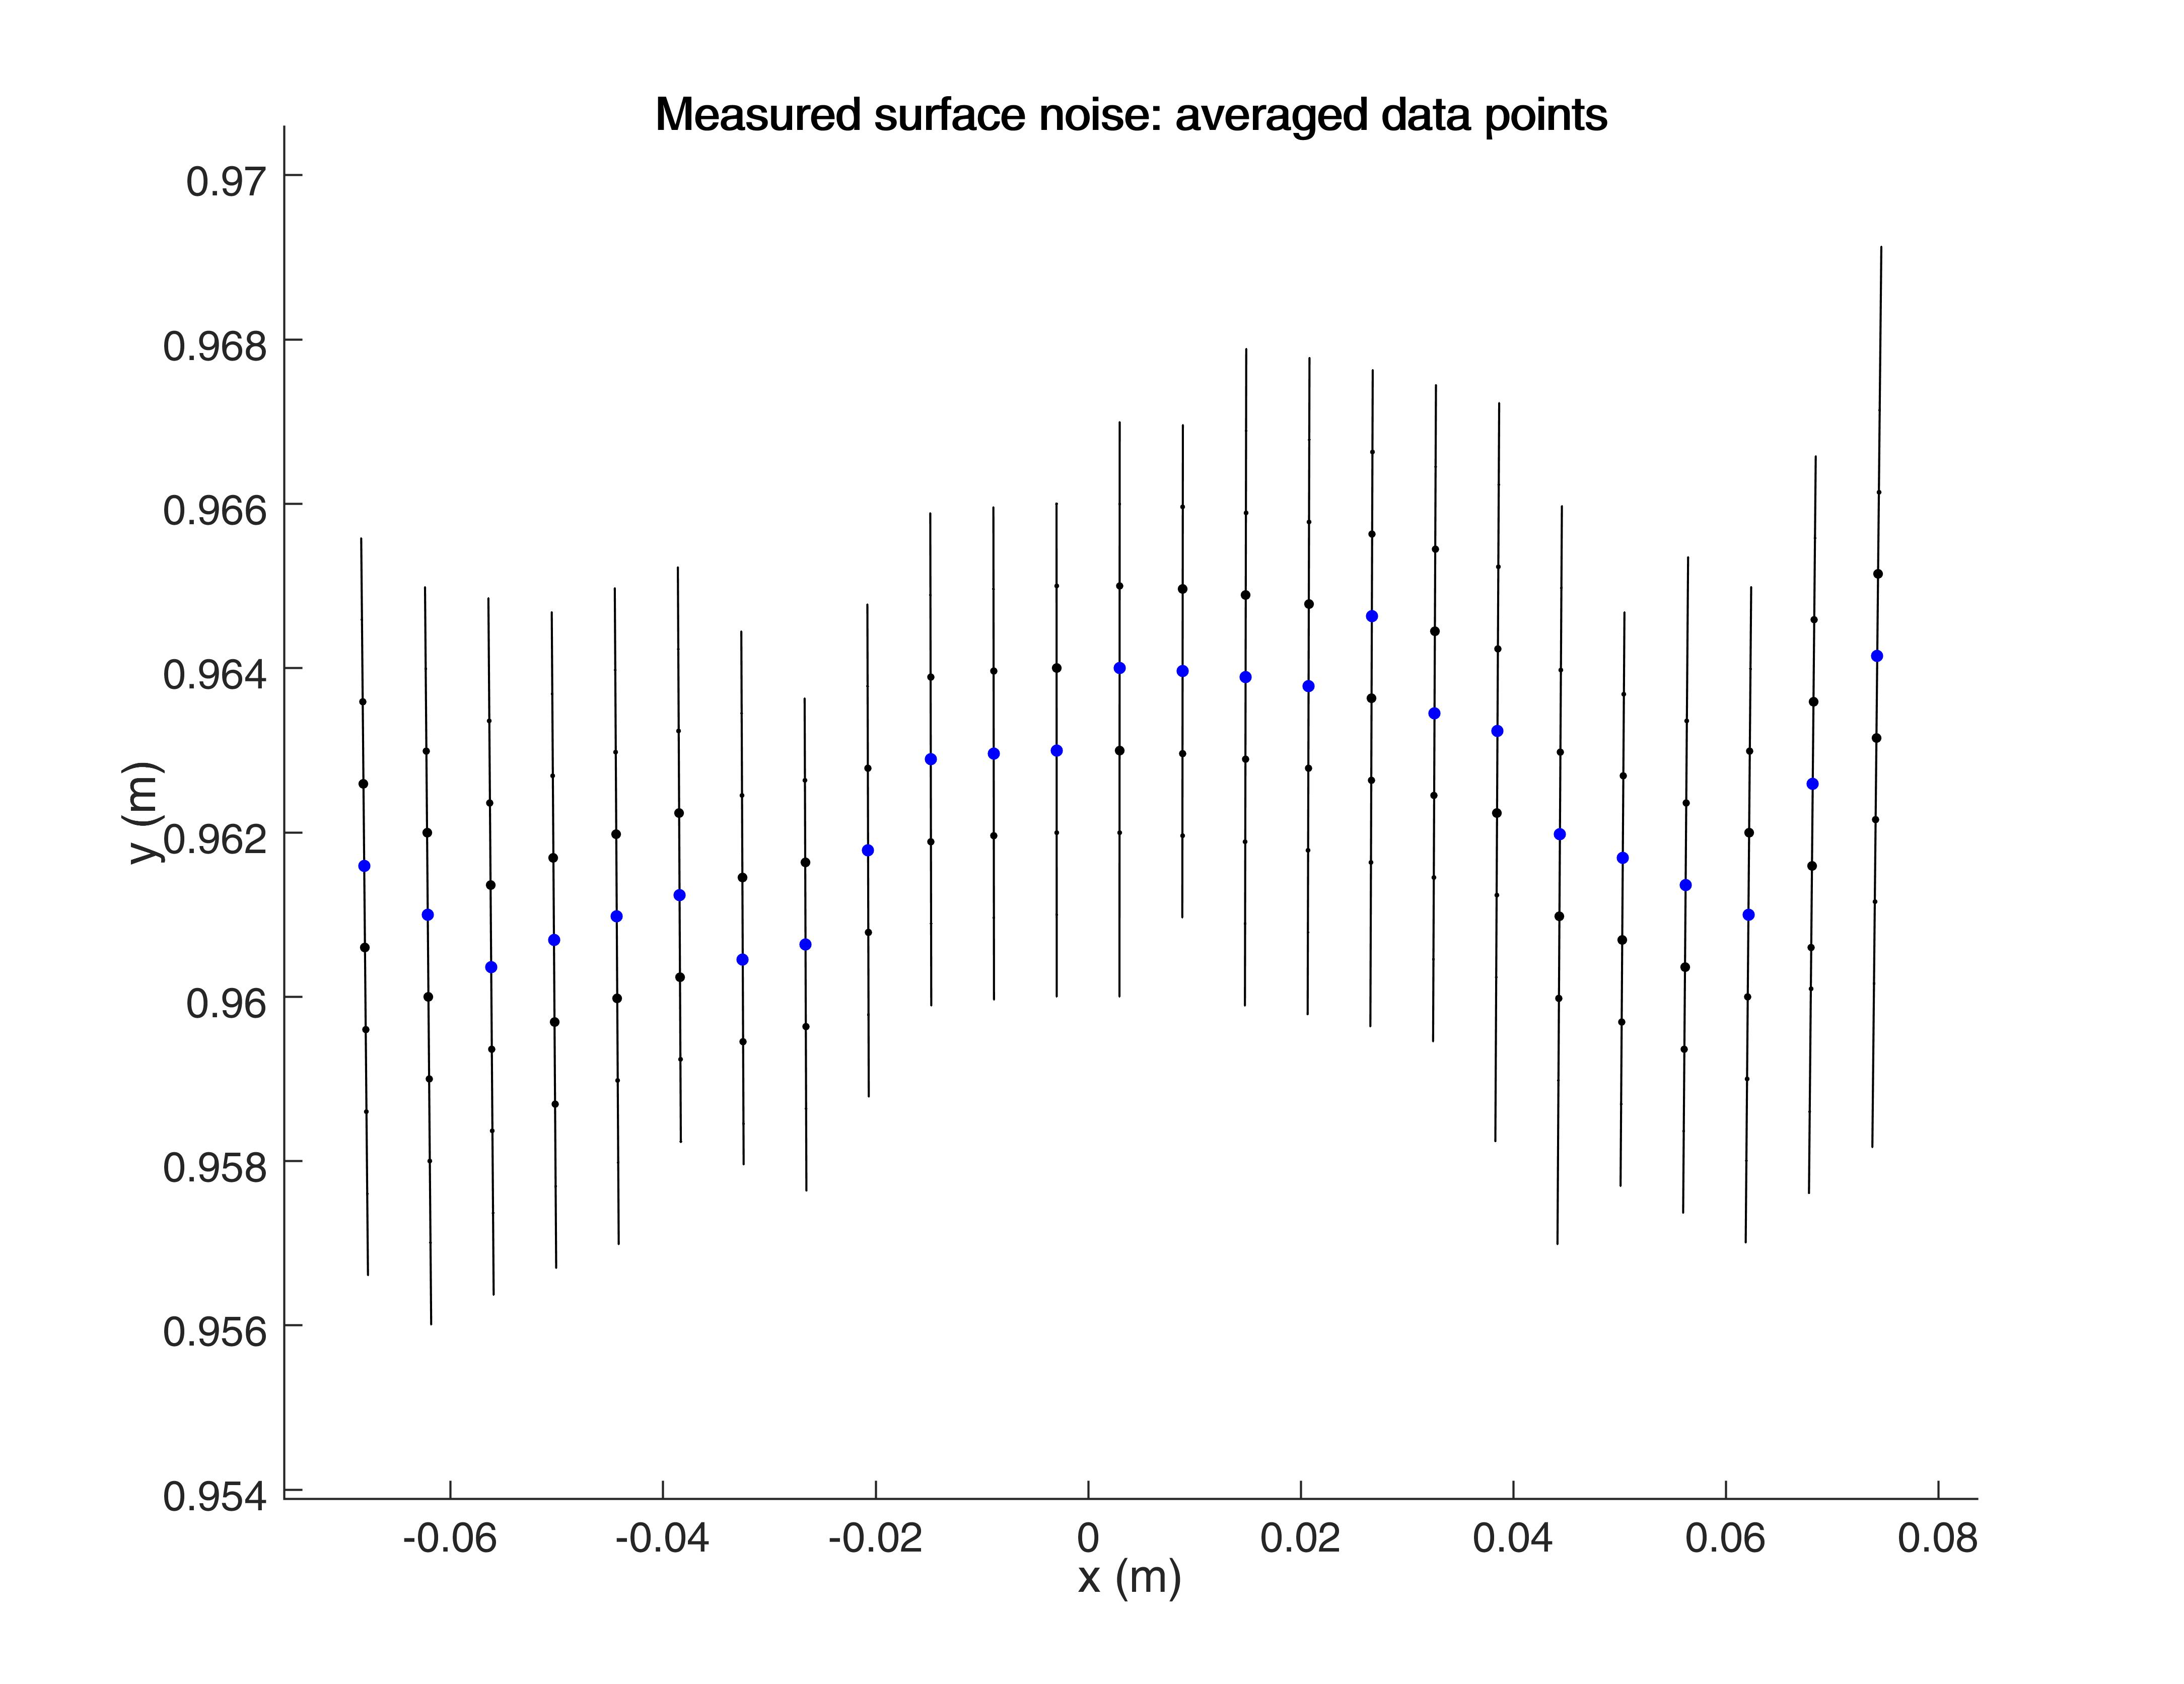
\includegraphics[width=1\textwidth,trim = 0mm 0mm 0mm 0mm,clip]{./Figures/measured_surface_noise}\vspace*{0ex}
	  		\end{minipage}}
	  		\subfigure[\label{fig:simulated_surface_noise}]{
	  		\begin{minipage}[b]{0.45\columnwidth}
    			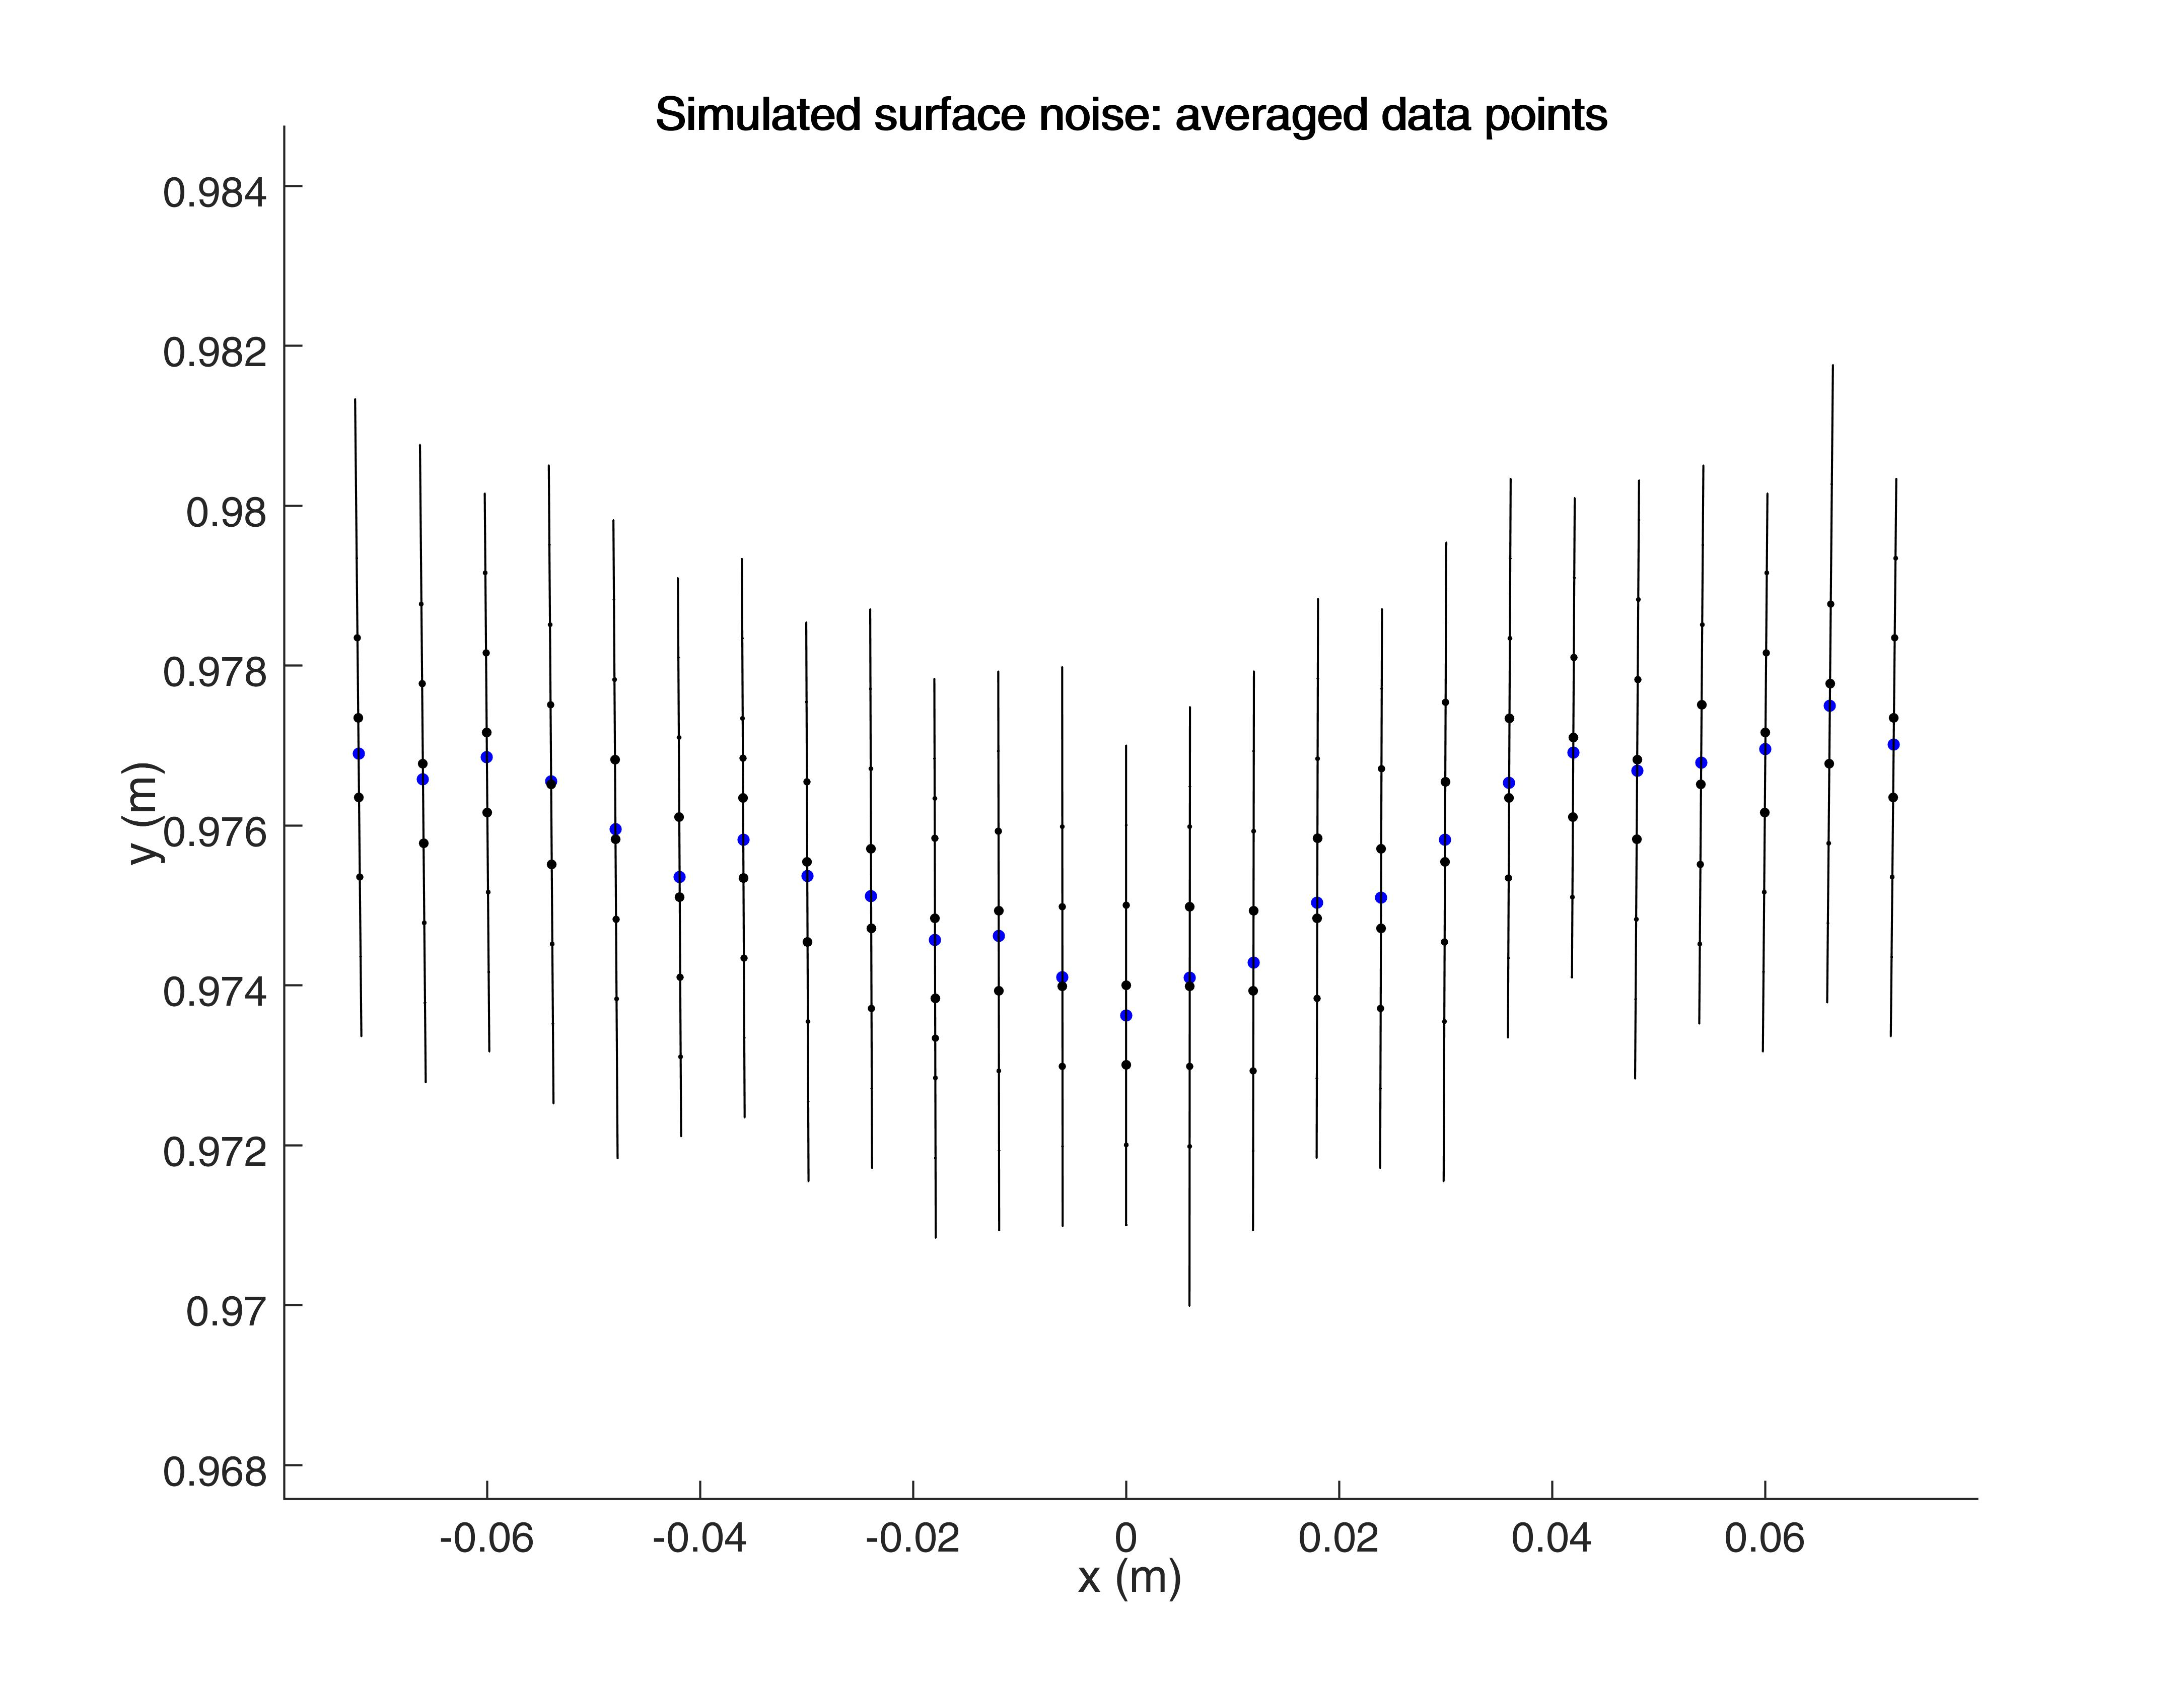
\includegraphics[width=1\textwidth,trim = 0mm 0mm 0mm 0mm,clip]{./Figures/simulated_surface_noise}\vspace*{0ex}
 			\end{minipage}}
	  		\caption{Comparision of (a) measured and (b) simulated surface noise}
	  		\label{fig:surface_noise}
		\end{figure}

\section{Testing Data Collection}
	\subsection{Setup}
		physical setup - PICS IN APPENDIX\\
		configurations/motions: \\
			-stationary\\
			-rotating\\
			-translating\\					
		arm forward kinematics $\rightarrow$ cube pose\\
		estimate sensor angle with horizontal with wall calibration data		
		
	\subsection{Results}
		still need to calibrate data.
		However, prediction is observer wont work. First, neither range or continuity assumptions will hold - gripper hold cube will mess with things. Lots of noise.
		Likely will need an infinite dimensional observer, estimate entire depth field. Need symmetry to get robust convergence.
		Still, data is available for future research.


\chapter{Conclusion}
 

\bibliographystyle{IEEEtran}
\bibliography{IEEEabrv,references}

\end{document}     